\documentclass[preprint,12pt]{elsarticle}
\usepackage{graphicx, xcolor, soul, eurosym, amsmath, float}
\usepackage{longtable, tabularx, booktabs, graphicx, subcaption, eurosym}
\usepackage{amssymb,amsthm, float, url,  newunicodechar, tikz}
\usepackage[utf8]{inputenc}
\usepackage{enumitem}
\usepackage{siunitx}
\sisetup{detect-all}
\graphicspath{{output/congested3/figures/}{output/congested3/}{output/paper-figures/}}
\newcolumntype{L}[1]{>{\raggedright\arraybackslash}p{#1}}
\newcolumntype{Y}{>{\raggedright\arraybackslash}X}
\newcommand{\var}[1]{\mathrm{#1}}
\usepackage[colorlinks=true,linkcolor=blue,citecolor=blue,urlcolor=blue]{hyperref} 
\makeatletter
\g@addto@macro{\UrlBreaks}{\UrlOrds}
\makeatother
\Urlmuskip=0mu plus 2mu\relax
\newunicodechar{−}{\ensuremath{-}}
\usetikzlibrary{
    positioning,  % node distance, right=of, below=of
    shapes.misc,  % rounded corners
    arrows.meta   % arrow heads
}

\newunicodechar{₂}{$_2$}
\makeatletter
\def\ps@pprintTitle{%
 \let\@oddhead\@empty
 \let\@evenhead\@empty
 \def\@oddfoot{\centerline{\thepage}}%
 \let\@evenfoot\@oddfoot}

\makeatother
% Re-designed by Sambeet

\begin{document}

\begin{frontmatter}

%% Title, authors and addresses

\title{Evaluating Data Centers as Local Energy System Assets: A System-Integrated PUE Approach}

\author[usn]{Sambeet Mishra}
\author[usn]{Ankana Singha}
\author[usn]{Khaled Aleikish}
\author[usn]{Thomas {\O}yvang}
\author[bax]{Dominic Stephen}
\author[srnl]{Rob Hovsapian}

\address[usn]{University of South-Eastern Norway, Porsgrunn, Norway}
\address[bax]{Bax Innovation, Barcelona, Spain}
\address[srnl]{Savannah River National Laboratory, USA}


\begin{abstract}
Data centers are becoming material actors in local electricity and heat systems. They are usually reported as large electricity consumers, but the same sites can also export waste heat, provide flexible load, and use storage to reduce stress on local networks. The difficulty is that the dominant operational metric, Power Usage Effectiveness (PUE), treats all non-IT electricity as overhead. A data center that installs heat pumps, heat exchangers, controllability, or storage can therefore look less efficient under PUE even when the design creates useful external value.

The paper first provides a contextual synthesis of policy, market, and project evidence on how data-center energy characteristics shape local business impacts in Europe. It then defines and tests the central contribution: \emph{A PUE-compatible companion indicator that converts separately accounted local-system benefits, including heat, flexibility, peak, carbon damage, and delay, into an energy-equivalent numerator credit.} We call this metric System-Integrated PUE (siPUE). The metric is tested in a two-stage design and operation framework with scenario-perfect benchmarks and a shared normalized min--max regret design. The min--max regret model serves as a disciplined uncertainty testbed for evaluating metric behavior. The model is evaluated for four archetypes and ten shared uncertainty states using annual representative-day profiles, a stylized three-node DC-OPF electricity network, heat-recovery constraints, lifecycle delay accounting, and a lease or opportunity-cost representation of land.

The canonical results separate the zero-investment identity case from the fair headline comparator. The identity no-services case has zero service capacity and zero efficiency investment, and verifies that siPUE reduces exactly to PUE. The headline comparison instead uses a constrained services-disabled comparator with the same locked 15\% efficiency retrofit and the same carbon-cap, network, land, delay, demand, and operational assumptions as the service-active cases. Averaged with each archetype weighted by annual IT energy, this fair comparator has PUE and siPUE of 1.167. The baseline design raises average PUE to 1.238 but lowers siPUE to 1.139, with 5.603~EUR/MWh IT of delay-adjusted system benefit. The robust design raises PUE further, to 1.343, and lowers siPUE to 1.152, with 10.825~EUR/MWh IT of delay-adjusted system benefit. Relative to the fair comparator, the baseline and robust credits are about 1.40 and 1.08 times their facility-energy burdens, respectively, showing diminishing marginal system value as integration intensity rises. At the scenario level, baseline siPUE is lower than the services-disabled comparator in 36 of 40 rows, while robust siPUE is lower in 23 of 40. Excluding carbon damage from the siPUE ledger reverses the IT-weighted average result for both service-active designs, so the conclusion is explicitly conditional on the stated social-carbon valuation. Train/test and out-of-sample diagnostics are internal verification and robustness checks; external validation would require observed project data.
\end{abstract}

\begin{keyword}
Data centers \sep Power Usage Effectiveness \sep System-Integrated PUE \sep waste-heat reuse \sep flexibility \sep robust optimization \sep local energy systems

\end{keyword}

\end{frontmatter}

\section{Introduction}
\label{sec:introduction}

Electricity demand from European data centers has become a material planning variable for both transmission and distribution networks. Commission estimates put EU consumption at 76.8~TWh in 2018, with projections of 98.5~TWh by 2030 under a trend scenario and up to 160~TWh under a high-growth case \cite{1}. More recent assessments suggest consumption already reached roughly 96~TWh in 2024 and could approach 168~TWh by 2030 \cite{2}.

Growth is reinforced by traffic expansion and a shift toward compute-intensive workloads. Artificial intelligence (AI) workloads are expected to accelerate demand, with energy needs rising rapidly during 2023--2030 \cite{3, 4}. AI also changes the temporal character of demand. Training and fine-tuning runs, batch pre-processing, model serving, and inference queues can shift facilities between accelerator-intensive training modes and latency-sensitive inference modes, changing IT power, heat rejection, cooling demand, and available flexibility headroom over operational timescales \cite{14,19}. The planning problem therefore extends beyond annual energy growth to how data-center operators and network planners manage ramps, peaks, and service availability.

If these trajectories persist, the data-center share of EU electricity could increase from about 3.1\% to around 5.7\% by 2035 \cite{2}, making aggregate demand comparable to national consumption in several member states \cite{5, 6}. At that scale, the build-out becomes a business and investment problem under binding local constraints: connection rights and congestion on the power side, offtake and tariff interfaces on the heat side, eligibility rules for flexibility markets, and land-use approvals, permitting timelines, and community acceptance at the site level increasingly shape which projects can proceed and how quickly capital can be deployed \cite{21}. Integration features can partially mitigate these frictions by delivering local co-benefits (e.g., heat export) or by reducing peak stress through controllability and storage, but they require additional interfaces and investment that must be evaluated on a comparable basis.

In parallel, the EU energy transition is pushing electricity and heat systems toward higher renewable shares, electrification, and sector coupling \cite{7}. Policy packages emphasize digitalization and flexibility as enabling layers for this transition \cite{8}, while sustainability reporting frameworks for large data centers are being formalized through Directive (EU) 2023/1791 and industry initiatives \cite{15, 16}. This setting creates a dual role for data centers: treated as inflexible loads they can exacerbate congestion, but when designed for integration they can supply valuable services such as waste-heat export and grid support \cite{11, 13, 22, 23}.

AI workload dynamics sharpen this dual role. At the grid interface, rapid load changes from clustered accelerators can appear as sub-second to minute-scale power swings, complicating voltage management, frequency regulation, and power quality. The same facility can also help manage those dynamics if batteries, controllable cooling, workload scheduling, and telemetry are organized to provide flexibility or peak relief \cite{8,13,Antal2018,Takci2025}. The value of such control is system-facing: it is created outside the conventional facility-efficiency boundary, even though the control hardware and cooling response may increase measured facility electricity.


Data-center participation in heat and flexibility markets is governed by tariffs, market access rules, and contract structures. Yet the dominant reporting metric, PUE, evaluates only internal electricity overhead and omits externally valued services. As a result, integration investments that increase electricity use to deliver heat, flexibility, ramp management, or reliability support can worsen reported efficiency even when they improve economic and system outcomes. This creates the KPI gap studied in this paper: PUE records the facility-energy burden of integrated control, while the separately accounted local-system benefit from managing dynamic loads, reducing peak stress, exporting heat, or supporting grid operation remains outside the metric. siPUE is introduced as a PUE-compatible companion indicator for translating those local-system benefits into the same energy-normalized language as PUE while preserving PUE's internal-efficiency role.

\subsection{Related Work}
\label{sec:related}

The literature relevant to this work spans five major areas:
(i) data centre efficiency metrics,
(ii) waste-heat recovery and district-heating integration,
(iii) data centre flexibility and demand response,
(iv) multi-energy integrated systems, and
(v) robust decision-making under uncertainty.
The first four streams are reviewed chronologically and highlight the metric gap that motivates System-Integrated PUE (siPUE); the fifth is reviewed separately because it grounds the Stage~2 optimization method used to test the metric definition.

\subsubsection{Foundation of Data Centre Metrics (2008--2012)}

The first generation of data centre metrics was established through
The Green Grid between 2008 and 2012, culminating in the widely adopted
Power Usage Effectiveness (PUE) metric \cite{Belady2008PUE, greengrid2014}.
PUE provided a simple ratio of total facility energy to IT energy and
played a crucial role in raising awareness about infrastructure
efficiency.
However, its design implicitly assumed that
(i) all non-IT energy is undesirable,
(ii) energy source differences are irrelevant, and
(iii) time-varying system behaviour is treated as irrelevant.
These assumptions became problematic as data centres began interacting
with electricity markets, district heating networks, and flexibility services.

\subsubsection{First Critical Analyses and Metric Extensions (2015--2017)}

By 2015--2017, several works began revealing structural weaknesses in
PUE.
Aravanis and Voulkidis \cite{Aravanis2015} highlighted the absence of
flexibility considerations.
Reddy et al.\ \cite{Reddy2017} provided a comprehensive taxonomy of
sustainability metrics and demonstrated that PUE captures only one
dimension of data centre performance.
Van de Voort et al.\ \cite{VandeVoort2017} showed empirically that PUE
varies with cooling architecture and climate, undermining fair
cross-facility comparisons.

During this period, additional single-dimension metrics emerged:
Carbon Usage Effectiveness (CUE), Water Usage Effectiveness (WUE), and
Energy Reuse Factor / Energy Reuse Effectiveness (ERF/ERE).
These standards (ISO 30134 series) addressed specific dimensions but
remained fundamentally parallel indicators, without a unified or
market-based way to aggregate them.

\subsubsection{Waste-Heat Recovery and District Heating Integration (2018--2020)}

Research into waste-heat utilisation expanded significantly as data
centres grew larger and more thermally intensive.
Early foundational work by Brunschwiler et al.\ \cite{Brunschwiler2011}
demonstrated the technical viability of high-grade heat recovery using
direct liquid cooling.
Wahlroos et al.\ \cite{11} analysed the integration of data
centre waste heat into Northern European district heating (DH) systems,
identifying substantial potential for system-wide carbon reductions.
Copertaro et al.\ \cite{10} positioned data centres as
prosumers that both consume electricity and export heat.
These works establish heat reuse as a genuine system service while leaving
open the need for an integrated metric capable of valuing it alongside
energy, carbon, or flexibility. The literature still lacks a reporting-compatible
way to translate heat export into an equivalent, market-aligned
sustainability score.

\subsubsection{Data Centre Flexibility and Demand Response (2019--2021)}

With increasing renewable penetration, data centres became candidates
for providing grid flexibility.
Liu et al.\ \cite{Liu2013} demonstrated how IT load modulation
(e.g., CPU scaling) can deliver demand response.
Antal et al.\ \cite{Antal2018} proposed an explicit flexibility
management framework for data centres.

However, these works analyse flexibility in isolation, without linking
it to heat reuse, carbon intensity, or facility-wide sustainability.
Furthermore, they often rely on engineering assumptions regarding
flexibility prices in place of settled service-specific market values.
This gap becomes evident in Crozier and Liska \cite{Crozier2025},
who find that real-world data centres exhibit weak price responsiveness,
highlighting the need for econometric estimation of flexibility value.

\subsubsection{Integrated Energy Systems and Sector Coupling (2020--2024)}

Research shifted toward integrated multi-energy systems around 2020.
Zhang et al.\ \cite{Zhang2022} surveyed the integration of data centres
with renewable energy.
Jerez Monsalves et al.\ \cite{JerezMonsalves2023} showed that flexible cooling
and waste-heat recovery from data centres reduce system costs and
emissions in the Danish energy system.
Wang et al.\ \cite{Wang2024} presented the ``Data Centre Integrated
Energy System'' (DC-IES) concept, combining electricity, heat, cooling,
renewables, and storage.

These studies quantify system-level impacts with economic valuation embedded
in optimisation models, leaving the standalone operator-indicator question open.

\subsubsection{Holistic Sustainability Metrics (2023--2025)}

Attempts to provide broader sustainability scoring emerged more recently.
Terenius \cite{Terenius2023} introduced the Datacenter Energy
Sustainability Score (DESS), which incorporates waste heat, energy
sources and social context.
DESS provides qualitative scoring and lacks market valuation or hourly
operational usability.
Newer reviews of waste heat \cite{Yuan2025, Hao2025} and data centre
flexibility \cite{Takci2025} reinforce the need for quantifiable,
energy-system-oriented indicators.

\subsubsection{Robust Decision-Making Under Uncertainty}

The two-stage design problem developed below is a robust-optimization exercise layered on top of the metric definition, drawing on a methodological literature outside the data-centre metrics streams above. Minimizing worst-case regret against a scenario-specific optimum is the minimax-regret criterion formalized by Savage \cite{savage1951theory} for decisions without a defensible single probability distribution over states -- the situation Knight \cite{knight2009risk} distinguishes from priced, distribution-known risk as genuine uncertainty. Lempert et al.\ \cite{MR-1626-RPC} operationalize this distinction for long-lived infrastructure planning, evaluating a shared design against a finite scenario ensemble and a worst-case robustness criterion in place of a single expected-value optimum; Stage~1 and Stage~2 in Section~\ref{sec:methodology} adopt the same structure, using scenario-perfect benchmarks and a shared worst-case-regret design while leaving the ten uncertainty states unweighted by probabilities. The secondary near-worst-case mean-cost tie-break used to resolve numerically degenerate ties at the worst-case optimum (Section~\ref{sec:methodology}) is a lexicographic scalarization, a standard device in multi-objective optimization for ranking a primary and secondary criterion without collapsing them into a single weighted objective \cite{Miettinen1999,Ehrgott2005,MarlerArora2004}. Framing Stage~2 this way clarifies the scope of the methodological claim: the paper uses an established minimax-regret criterion as a controlled testbed for observing how siPUE and PUE respond to the same design choice under uncertainty.

\subsection{Synthesis and Gap Identification}

Table~\ref{tab:metric-novelty-comparison} positions the proposed metric against the closest reporting metrics and integrated-system modelling literature. The contribution lies in the accounting translation from local-system value into a PUE numerator credit.

\begin{table}[tbp]
\centering
\scriptsize
\setlength{\tabcolsep}{3pt}
\renewcommand{\arraystretch}{1.12}
\caption{Comparison of siPUE with adjacent data-centre metrics and modelling approaches.}
\label{tab:metric-novelty-comparison}
\begin{tabularx}{\linewidth}{L{2.05cm} L{2.25cm} L{1.65cm} L{1.85cm} Y}
\toprule
Approach & Primary function & Values local-system services? & PUE numerator credit? & Gap relative to siPUE \\
\midrule
PUE \cite{Belady2008PUE,greengrid2014,EUDataCenterDirective2023} & Facility electricity divided by IT electricity & No & Baseline ratio & Treats heat-pump, storage, and control electricity as overhead even when they create external value. \\
ERF/ERE \cite{EUDataCenterDirective2023} & Reused-energy reporting and energy-reuse effectiveness & Heat only, in energy terms & Partial reuse adjustment & Omits flexibility, peak, network, carbon-damage, and delay effects. \\
CUE \cite{Reddy2017} & Carbon emissions per IT energy & Carbon footprint only & No & Parallel carbon-intensity indicator outside the PUE-compatible local-system credit. \\
WUE \cite{EUDataCenterDirective2023} & Water consumption per IT energy & No & No & Tracks water use outside the energy-system value boundary. \\
REF \cite{EUDataCenterDirective2023} & Renewable-energy share & No & No & Tracks procurement mix; local heat, flexibility, peak, carbon-damage, and delay value remain outside its boundary. \\
DESS \cite{Terenius2023} & Broader sustainability score & Partial, contextual & No & Qualitative and contextual metric with limited market-valued PUE compatibility. \\
DCRE \cite{GreenGrid2025DCRE} & Resource-effectiveness view of energy, water, water stress, and climate context & Indirect & No & Broader resource metric outside PUE numerator-credit reporting. \\
Integrated energy-system optimisation papers \cite{JerezMonsalves2023,Wang2024} & System-cost or emissions optimisation & Yes, inside the model & No & Quantifies system impacts while leaving standalone reporting-compatible numerator credits undefined. \\
siPUE (this study) & Companion indicator for service-active data centres & Yes: heat, flexibility, peak, carbon damage, and delay & Yes & Converts separately accounted local-system benefit into an energy-equivalent numerator credit and reduces to PUE in the no-services identity case. \\
\bottomrule
\end{tabularx}
\end{table}

Across this literature, three persistent gaps remain:

\begin{itemize}
\item Fragmentation: The reporting metrics reviewed here (PUE, CUE, WUE, ERF/ERE, REF, DESS, DCRE) each measure one dimension or resource bundle, leaving local-system services without a PUE-compatible companion score
\item Lack of market valuation: Heat reuse, flexibility, and carbon impacts are rarely valued using empirical electricity, heating, reserve or ETS price data; most studies rely on engineering assumptions or ad hoc pricing
\item Absence of a PUE-compatible local-system credit: Among the approaches reviewed here, we did not identify a transparent numerator credit that converts separately accounted heat, flexibility, peak, carbon-damage, and delay effects into the same energy-normalized language as PUE
\end{itemize}

\subsection{Conceptual Framework and Research Questions}
The paper is structured around a conceptual framework that links energy characteristics, data center design decisions, and local energy system outcomes. 
Evidence from policy documents, market data, and industry practice provides qualitative and institutional context for the energy characteristics and business readiness layer, while the model formalizes the data center responses and quantifies system outcomes. Section~2 is therefore treated as contextual synthesis rather than a standalone structured-review result. This leads to the following model-facing research questions:
\begin{enumerate}
\item RQ1: Can a PUE-compatible companion indicator reveal local-system value from heat, flexibility, peak, carbon damage, and delay while preserving the no-services PUE identity
\item RQ2: How do robust, cost-minimizing design decisions shift traditional efficiency metrics and system-integrated indicators
\end{enumerate}

The remainder of the paper first provides the contextual synthesis, and then addresses RQ1--RQ2 through the metric definition and model-based analysis.

\subsection{Contributions}
This paper makes four contributions:
\begin{enumerate}
\item It integrates evidence on data centers and local energy systems, emphasizing how energy characteristics, AI workload dynamics, and integration options shape local business impacts and investment readiness.
\item It defines and tests siPUE as an accounting bridge between PUE's facility-energy burden and separately accounted local-system benefits.
\item It uses a two-stage optimization model with scenario-perfect benchmarks and a shared normalized min--max regret design as the uncertainty testbed for evaluating the metric, with lifecycle delay, carbon ledgers, land accounting, heat recovery, flexibility, storage, and DC-OPF network constraints.
\item It evaluates siPUE for four archetypes and ten shared uncertainty states, reports the PUE--siPUE value-channel result, decomposes the siPUE credit by ledger component, and tests sensitivity to the reference price, heat price, flexibility price, cooling overhead, land availability, and construction delay.
\end{enumerate}

\section{Data Centers in Local Energy Systems --- Policy and Market Context}

This section examines how data centers interact with local energy systems from a policy and business-investment perspective. Data-center electricity use has become a material planning variable in Europe. Commission assessments place EU consumption at 76.8~TWh in 2018, with projections of 98.5~TWh by 2030 under a trend case and up to 160~TWh under a high-growth case \cite{1}. Industry reporting suggests that demand already reached roughly 96~TWh in 2024 and could approach 168~TWh by 2030 \cite{2}. These trajectories are driven by sustained cloud growth, accelerating data traffic, and the energy intensity of AI workloads \cite{3,4,14}. At the facility level, non-IT energy remains significant; cooling and auxiliary systems typically account for roughly 30--40\% of total electricity consumption \cite{19}. The combination of scale and growth means that data-center siting and design decisions now shape local grid planning and regional investment pipelines.

At the same time, Europe is pursuing decarbonization, electrification, and sector coupling, which require more flexible and digitally coordinated energy systems \cite{7,8,9}. Data centers are large loads and potential local system assets that can provide waste-heat recovery, flexible demand, and grid services when integration pathways exist. This duality creates a business challenge: integration can unlock new revenues and de-risk grid access, while also adding capital costs and exposing projects to policy and market uncertainty.

This section therefore adopts an explicitly business-oriented lens. The macro--meso--micro structuring adopted in this study is informed by the multi-level perspective (MLP) on socio-technical transitions \cite{GEELS2020119894}. Projects must reach financial close under uncertainty about connection rights, tariff treatment, reporting requirements, and partner commitments. The multi-level governance framework is used to explain how data-centre innovations can scale into broader socio-technical transitions. Micro-level projects generate learning and proof of concept, meso-level actors (e.g., utilities and regional authorities) enable replication through rules and delivery models, and macro-level policy and funding shape long-term direction. This lens fits the data-centre context because scaling depends on technology, enabling policies, workable organisational models, and access to low-cost, standardised finance. The analysis is organized around (i) binding constraints that shape site selection and time-to-market, (ii) the service channels that enable value stacking, and (iii) the cross-level governance conditions that determine whether integration becomes bankable. This framing motivates why a reporting-compatible metric that accounts for externally valued services is needed for coherent investment and performance assessment.


The investment case for system-integrated data centers is shaped by interlocking constraints that operate at different governance levels. Macro policy establishes regulatory certainty and carbon-price trajectories; meso infrastructure determines physical feasibility and sequencing; micro finance translates the resulting risk profile into capital costs and revenue requirements. These layers interact. Policy can create incentives that lower financing costs, but only if local infrastructure exists to deliver services and project-level contracts can lock in revenue.

\subsection{Macro level --- Policy and market architecture}
The macro level refers to EU and national policy priorities, regulation, and funding frameworks that shape incentives for data-centre energy integration. Stakeholders include EU institutions, national ministries, regulators, and public funding bodies. At the macro level, EU climate policy provides the overarching regulatory frame for integration. The European Green Deal and the ``Fit for 55'' package establish binding decarbonization targets that indirectly increase the value of electricity efficiency, waste-heat reuse, and flexibility services \cite{17,7}. The Energy Efficiency Directive recast (Directive (EU) 2023/1791) introduces explicit reporting obligations for large data centers and codifies sustainability KPIs such as PUE, Renewable Energy Factor, and Energy Reuse Factor \cite{15,EUDataCenterDirective2023}. Voluntary commitments such as the Climate Neutral Data Centre Pact reinforce these objectives and translate them into sector-level targets for renewable supply and heat reuse \cite{16}. These policy instruments matter as compliance obligations and governance signals: reporting metrics become part of lender and investor due diligence, shaping reputational risk, access to capital, and eligibility for public support.

Standardized KPI disclosure also functions as a capital signal. Reporting comparability affects ESG scoring, due diligence, and financing conditions. Where reporting frameworks emphasize internal efficiency without recognizing system services, integration investments may appear less performant despite improving system outcomes\cite{15,16,EUDataCenterDirective2023,greengrid2014}. This misalignment between public objectives and private performance metrics can weaken incentives for system-integrated design.

Digitalization policy is the second macro pillar. The EU action plan for digitalizing the energy system frames flexibility, interoperability, and data availability as prerequisites for integrating variable renewables and coordinating distributed assets \cite{8}. This positions data centers as potential ``digital-energy hubs'' whose operational telemetry, controllability, and digital interfaces are integral to system services. Macro-level policy thus creates an incentive landscape in which data centers that can provide measurable services are more likely to qualify for preferential treatment or supportive tariffs, while those that remain inflexible loads face higher regulatory risk or stricter connection conditions.

Policy-induced investment incentives sit alongside these reporting obligations. Regional initiatives and public--private programs aim to accelerate investment readiness by providing blueprints, de-risking mechanisms, or bundled project pipelines \cite{18,interregnorthseaBRAVEBuilding}. The business impact of such programs depends on their stability and on whether they can shorten the time to contract and commissioning. Where incentives are credible and durable, they reduce financing risk; where they are uncertain, they can amplify the option value of waiting.

Carbon pricing adds a third macro channel. The EU ETS has measurable impacts on electricity-system dispatch and price formation, with carbon price trajectories shaping the relative value of demand reduction, heat reuse, and electrified heat pumps \cite{Xu2023}. For data centers, carbon exposure becomes a regulatory risk that influences the expected marginal cost of electricity and the value of low-carbon energy supply. This policy risk also has a financial channel: it affects the discount rates applied to future cash flows and the choice between integration investments and conventional efficiency upgrades. A stable carbon-price trajectory can support long-term contracts for heat and flexibility; a volatile trajectory increases revenue uncertainty and can delay investment.

Regulatory certainty compounds across these macro channels: because data centers are long-lived assets, durable policy signals reduce financing risk while volatile signals raise it\cite{7,15,16}, a dynamic developed in financial detail at the micro level below.

Finally, electricity market design determines whether flexibility can be monetized and whether congestion relief is rewarded. Studies on data-center flexibility show that market access and product design are decisive for realizing value from demand response and ancillary services \cite{12,13,Takci2025,Crozier2025}. Where balancing markets are open and telemetry requirements are feasible, data centers can monetize battery and load flexibility. Where participation rules are opaque or markets are illiquid, flexibility has limited bankability. Macro policy sets the boundary conditions for value stacking; investable outcomes still depend on local access rules and contracts.

\subsection{Meso level --- Regional infrastructure and spatial constraint}
The meso level covers regional and local governance and market arrangements that turn policy into planning, tariffs, and investable projects. Stakeholders include regional/metropolitan authorities, DSOs/TSOs, district-heating operators, aggregators, and local permitting bodies. Meso level conditions determine whether macro incentives can be converted into projects. The binding constraint is often grid capacity more than annual energy. Large, near-constant loads can trigger network reinforcements, and in some regions grid operators have constrained or paused new data-center connections due to local network limits \cite{21}. Congestion pricing and connection-rights frameworks influence both operating costs and the feasibility of additional load, making grid access a strategic asset. Regional transmission and distribution operators increasingly treat large data centers as sources of local stress, which means that permitting and connection rights depend on credible mitigation strategies and co-benefits \cite{6,21}. This logic directly affects capital allocation: projects with grid-relief features (flexibility, behind-the-meter storage, or verifiable heat export) are more likely to clear permitting and avoid costly grid upgrades.

Congestion is a planning, pricing, and contract issue. Where congestion charges or locational tariffs are applied, the effective electricity cost can vary materially across sites and over time, and grid import caps can become binding constraints that limit expansion options. These locational signals influence both revenue projections and risk assessments, especially for projects that rely on tight operating margins. For developers, the implication is that congestion relief and flexibility can carry real option value by protecting against future price volatility and curtailment risk \cite{6,21}.

Permitting and local acceptance further tie congestion and land constraints to business outcomes. Municipalities increasingly evaluate data-center projects through the lens of local co-benefits, including heat reuse, grid services, or renewable integration. Projects that can credibly demonstrate such co-benefits often face lower permitting friction and stronger stakeholder support. This turns integration into a strategic permitting asset.

Land is a parallel constraint. Large facilities require substantial plots, and integration equipment---heat pumps, heat exchangers, thermal storage, battery containers, and electrical substations---expands the footprint and the need for utility corridors. Land availability is both a physical and capital constraint: siting in land-scarce zones raises acquisition costs, extends permitting timelines, and forces trade-offs between integration depth and real-estate feasibility. Because location choices are sticky, land constraints create spatial lock-in: once a site is committed, the ability to exploit local heat networks, renewable resources, or grid capacity is fixed for the project's life. This lock-in is especially relevant for projects that require proximity to district heating networks or industrial offtakers to monetize waste heat \cite{22,23}.

Land constraints also shape expansion options. Integrating heat recovery, storage, or on-site substations often competes with future IT expansion or with other land-intensive infrastructure such as logistics or water-treatment systems. In urban or industrial clusters where land prices and zoning restrictions are tight, these trade-offs can shift investment decisions toward smaller integration packages or phased deployments. The business implication is that land functions as a capacity-limiting factor that affects both near-term financing and long-term optionality.

District heating infrastructure is a second meso constraint. Heat reuse is technically feasible in many contexts, but commercial viability depends on network proximity, temperature requirements, and utility tariff structures \cite{10,11,22,23}. In regions with established district-heating governance, standardized interconnection rules and repeatable contract templates reduce transaction costs and improve bankability \cite{11,23}. In regions without such infrastructure, heat recovery becomes a long-lead investment requiring coordination across municipalities, utilities, and private developers. These differences fall outside a single efficiency metric and directly influence capital requirements and revenue timing.

Infrastructure sequencing is central to this coordination challenge. Heat recovery projects often require parallel investments in heat-pump capacity, pipework, and network reinforcement. When the heat network expands more slowly than data-center build-out, the heat revenue stream is delayed or curtailed, which weakens the business case and can strand integration assets. Successful projects typically resolve sequencing risks through early-stage agreements on expansion schedules and tariff treatment, often involving municipal utilities as coordinating agents. This sequencing constraint mirrors grid reinforcement delays and reinforces the need to price construction delay and infrastructure timing explicitly in investment analysis.

Renewable resource geography also shapes meso feasibility. Nordic contexts provide lower ambient temperatures and proximity to low-carbon generation, improving both PUE performance and the economics of heat cascading \cite{24}. Conversely, high-demand urban clusters often combine strong heat demand with constrained grid capacity and scarce land, raising the value of integration while making it harder to realize. Emerging ``energy hub'' concepts co-locate data centers with renewables, storage, and other flexible loads, using the data center as anchor demand to unlock investment in local generation \cite{25}. These spatial factors make site selection a strategic business decision shaped by technical constraints.

Construction delay is the critical meso-level risk that links infrastructure constraints to financial outcomes. Grid reinforcements, zoning approvals, and interconnection negotiations can delay energization even when a facility is otherwise ready, creating a timing asymmetry between developers and network operators. Because data centers are capital intensive, delays destroy value by shifting revenue streams without reducing fixed costs. The risk is amplified when integration assets are built ahead of guaranteed market access or offtake contracts, which can strand capital for multiple years. This makes infrastructure sequencing and partner coordination central to investment readiness.

Timing asymmetry is particularly acute when grid reinforcement timelines exceed data-center construction timelines. In many jurisdictions, data centers can be built in 18--24 months, while network upgrades or district-heating expansions require multi-year planning cycles. This mismatch creates a coordination risk: capital can be deployed faster than enabling infrastructure, and the resulting idle capacity erodes IRR and reduces appetite for integration. The report highlights that successful projects often rely on early-stage alignment between developers, utilities, and municipalities to synchronize these timelines and to lock in connection rights before major capital is committed.

\subsection{Micro level --- Project finance and capital allocation}
The micro level refers to site-level technologies and contracts implemented by individual data centres and their partners. Stakeholders include data-centre operators, technology providers, heat off-takers, flexibility/market participants, and on-site energy service companies. At the micro level, investors evaluate data centers through cash-flow logic: Net Present Value (NPV), Internal Rate of Return (IRR) thresholds, and the ability to service debt under downside scenarios. Integration investments increase upfront CAPEX (heat pumps, exchangers, storage, telemetry), but can diversify revenue by adding heat-offtake and flexibility payments to the core IT business. The report highlights that diversified business models are central to investment readiness, particularly when heat and flexibility revenues are structured as contracted cash flows with limited speculative market exposure. Evidence from European heat-reuse projects shows that commercial structures range from utility-paid offtake contracts to co-investment models, with long-term price agreements often required to reach bankability \cite{23}. On the flexibility side, value capture depends on market access and the ability to meet telemetry and performance requirements \cite{12,13}.

Uncertainty increases the cost of capital. If energy prices, carbon prices, or market-access rules are unstable, investors apply higher discount rates or require stronger contractual guarantees. This raises the hurdle for integration assets relative to conventional efficiency upgrades. Delay risk exacerbates this effect: construction delays lengthen the period before revenue accrues and can breach debt-service covenants. The option value of waiting can therefore dominate near-term integration decisions, especially when the regulatory trajectory or grid-reinforcement timetable is uncertain. These dynamics make financing conditions as important as technical feasibility.

Debt structure and covenant design translate these uncertainties into capital allocation decisions. Projects that can demonstrate long-term contracted heat offtake or stable flexibility revenues are more likely to access lower-cost debt and higher leverage, while projects with speculative service revenues face equity-heavy structures and higher required returns. Integration therefore creates a trade-off: it raises CAPEX but can reduce long-run risk if service contracts are credible. This trade-off is central to investment appraisal and underpins the need for metrics that translate system-service value into signals that financiers can use.

Performance metrics influence financing costs. Reporting obligations under the Energy Efficiency Directive and voluntary sector commitments institutionalize PUE and related KPIs as governance tools \cite{15,16}. Because lenders and investors increasingly rely on standardized metrics in ESG scoring and due diligence, KPI performance can affect the cost and availability of capital. The challenge is that conventional PUE treats all non-IT electricity consumption as overhead, which can penalize projects that add integration assets to generate external system value \cite{greengrid2014,Belady2008PUE,VandeVoort2017}. This creates a micro-level financing risk: projects that improve system outcomes may appear worse on standard metrics, potentially raising financing costs despite stronger long-term value.

These financing dynamics incentivize staged integration strategies. Developers may prioritize assets that secure connection rights or heat offtake first, while deferring optional assets (e.g., additional storage or advanced controllability) until market access or tariff structures are clearer. Integration becomes bankable when uncertainty is reduced through contracts, regulatory clarity, or pilot-scale validation. The model developed below reflects this reality by separating regimes with active services from those where integration remains latent.

These characteristics imply that data centers simultaneously represent infrastructure pressure and integration opportunity. The following section conceptualizes the primary service channels through which integration occurs.

\subsection{Service Channels and Revenue Stacking}

Data centers contribute to local energy systems through three principal channels: heat recovery, electrical flexibility, and coordinated renewable anchoring. These channels correspond to potential value streams that can be stacked to improve project economics, but each requires distinct infrastructure interfaces, market access conditions, and contractual arrangements. The business relevance is direct: contractible and measurable service revenues can offset integration CAPEX and reduce dependence on volatile electricity prices; weak revenue recognition can push integration toward compliance-cost treatment.

Financing structures tend to mirror these revenue profiles. Where long-term offtake or flexibility contracts are in place, projects can access cheaper debt and higher leverage; where revenues are uncertain, equity shares increase and hurdle rates rise. The business consequence is that integration decisions depend on contract design and counterparty risk. Bankable integration often requires early-stage negotiation with utilities and municipalities so service revenues enter the financial model as contracted cash flows.

Measurement and verification are an additional, often underestimated, business requirement. Heat export requires calibrated metering and agreed accounting for temperature lift and losses; flexibility participation requires real-time telemetry and compliance with market performance metrics \cite{8,13}. These systems impose capital and operational costs that need to be internalized in the financial model. The EU digitalization action plan explicitly positions interoperable data standards and monitoring infrastructure as enabling conditions for flexibility and sector coupling \cite{8}. For data centers, this implies that integration is partly a data-governance investment: robust measurement and reporting systems make service revenues settleable and verifiable, reducing financial risk.

Data centers reject low-grade heat that can be recovered from cooling circuits and upgraded for productive use. In a common configuration, a secondary water loop extracts heat via an exchanger and provides a low-temperature source stream (typically in the 25--40$^\circ$C range) that is lifted by a heat pump to district-heating supply levels or used by nearby process-heat offtakers.

Figure  \ref{fig:heat-mechanism} illustrates the physical and contractual structure of this service channel. The upper layer represents the thermodynamic pathway from IT load to heat delivery. The lower layer highlights the institutional interface required for monetization: connection to district heating infrastructure and contractual alignment with utilities or local offtakers.
\begin{figure}[t]
\centering
\footnotesize
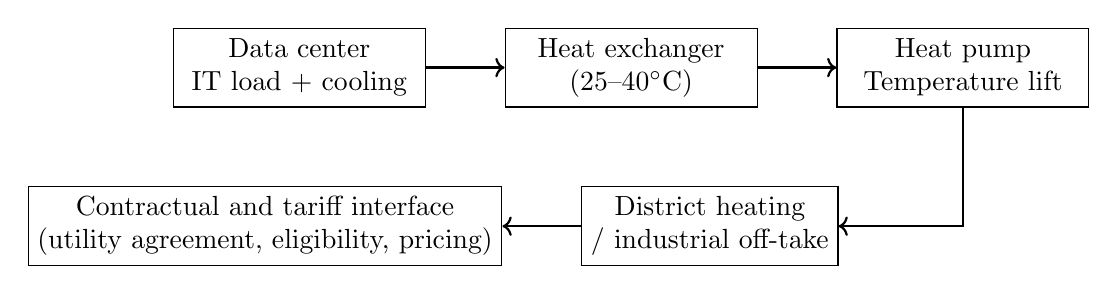
\begin{tikzpicture}[
box/.style={rectangle, draw, align=center, minimum width=3.2cm, minimum height=1.0cm},
arrow/.style={->, thick}
]

% Top row
\node[box] (dc)
{Data center\\
IT load + cooling};

\node[box, right=1cm of dc] (hx)
{Heat exchanger\\
(25--40$^\circ$C)};

\node[box, right=1cm of hx] (hp)
{Heat pump\\
Temperature lift};

% Bottom row (shifted left)
\node[box, below=1cm of hx, xshift=1cm] (dh)
{District heating\\
/ industrial off-take};

\node[box, left=1cm of dh] (contract)
{Contractual and tariff interface\\
(utility agreement, eligibility, pricing)};

% Arrows
\draw[arrow] (dc) -- (hx);
\draw[arrow] (hx) -- (hp);
\draw[arrow] (hp) |- (dh);
\draw[arrow] (dh) -- (contract);

\end{tikzpicture}
\caption{Process flow for recovery and upgrading of data centre waste heat for district heating or industrial off-take, including the contractual and tariff interface.}
\label{fig:heat-mechanism}
\end{figure}


Urban waste heat has been identified as a material resource for decarbonizing building heating when effectively integrated \cite{22}. The recast Energy Efficiency Directive introduces reporting and feasibility assessment obligations for large facilities \cite{15}. However, economic viability depends on tariff structures, network access, regulatory certainty, and technical feasibility together.

A large share of data-center waste heat is technically recoverable under suitable configurations, but monetization pathways are uneven across regions. Even where heat demand exists, mismatch between seasonal demand, temperature requirements, and network access can reduce achievable utilization factors. From a business perspective, the decisive variables are heat availability, long-term offtake commitments, and the allocation of temperature-lift responsibilities across stakeholders (operator, utility, or third-party owner).

Financing structures reinforce this point. Heat-recovery assets often sit outside the data-center ``fence line'' and require co-investment with utilities or municipalities. In practice, bankable projects rely on long-term contracts that define pricing, curtailment rules, and performance obligations, which transforms heat export from an uncertain byproduct into a predictable revenue stream \cite{23}. Where such contracts are absent, heat recovery is treated as discretionary, even if it improves system outcomes.

Project evidence indicates that heat recovery can be commercialized through multiple arrangements: utility-paid offtake into district heating, co-investment in heat pumps and network interfaces, or third-party ownership of the recovery assets with long-term heat purchase agreements. Best-practice surveys document operational and late-stage projects across diverse European contexts, suggesting that remaining barriers often concern institutions, interconnection terms, tariff treatment, and responsibility allocation \cite{23}. In regions with mature district-heating governance, standardized interconnection rules and repeatable contract templates reduce transaction costs and improve investment readiness \cite{11,23}.

Successful heat projects typically emerge where municipal utilities, developers, and offtakers coordinate early on tariffs and network expansion. Examples from Nordic and Central European cities show that heat reuse becomes commercially viable when district-heating operators can monetize lower-temperature supply and when data centers can internalize a share of the avoided heat costs. These cases place heat recovery at the intersection of policy, infrastructure, finance, and multi-actor contracting \cite{23}.

Heat pricing is often indexed to local fuel prices or to regulated district-heating tariffs, which means that the business value of heat export depends on broader energy-market conditions and carbon pricing. As carbon prices rise, the relative value of low-carbon heat increases, improving the economics of heat recovery even when electricity costs rise \cite{Xu2023}. For data centers, this introduces a second price exposure beyond electricity: the heat price trajectory. This reinforces the importance of long-term offtake agreements that define price indexation and risk sharing between operators and utilities \cite{22,23}.

Beyond thermal integration, data centers possess latent flexibility through controllable loads and battery systems originally installed for reliability. Under appropriate market rules, these assets can provide balancing and ancillary services \cite{13}. Estimates suggest that European data centers could offer substantial demand response capacity if enabled by market design \cite{12}. Demonstrated deployments illustrate that portions of battery capacity can participate in balancing markets without compromising uptime \cite{14}.

Flexibility participation depends on both technical capability and regulatory access. On the technical side, controllable cooling and workload shifting allow short-term reductions in demand without service disruption, while battery energy storage provides fast response for frequency regulation or reserve products \cite{13,Antal2018,Takci2025}. On the regulatory side, eligibility criteria, telemetry requirements, and settlement intervals determine whether data centers can participate at scale \cite{Crozier2025}. Where these conditions align, flexibility can become a stable revenue stream that also reduces congestion and improves permitting prospects.

The business logic is therefore twofold: flexibility can generate direct market revenue, but it can also serve as a strategic asset for grid access and risk mitigation. This dual role strengthens the case for system-integrated operation in congested regions, yet it remains invisible to traditional efficiency metrics.

From a revenue perspective, flexibility can be decomposed into distinct products with different risk profiles: short-duration frequency regulation, reserve capacity, and longer-duration demand response or arbitrage. Each product entails specific telemetry and performance obligations, which affects participation costs and contractual design \cite{13,Takci2025,Crozier2025}. The operational implication is that a data center may need to dedicate specific assets to market participation, which introduces opportunity costs that must be reflected in investment analysis.


Renewable integration occurs through both procurement and physical coupling. Many operators rely on corporate power purchase agreements or other instruments to match annual electricity use with renewable generation, while siting decisions increasingly favor regions with low-carbon supply and available network capacity. At the meso level, emerging ``energy hub'' concepts co-locate data centers with renewables, storage, and other flexible loads, using the data center as an anchor demand and a controllable participant in local balancing \cite{25}. Demonstration projects in Nordic contexts also illustrate how clean generation and cold climates can support both lower overhead and novel energy-cascading uses of waste heat \cite{24}.

Smart local energy system concepts emphasize the value of coordinated, place-based integration that aligns generation, storage, and demand \cite{9}. Data centers are well positioned to act as anchor loads within such systems because they provide stable demand and can deploy digital control for flexibility. Local energy communities and regional innovation ecosystems are increasingly exploring these configurations, but their success depends on governance arrangements that allocate benefits across utilities, municipalities, and operators. As a result, renewable coordination is as much an institutional and contractual challenge as a technical one.

From a business perspective, renewable coordination can reduce exposure to wholesale price volatility and strengthen ESG positioning, but it also binds projects to specific geographies and infrastructure timelines. In practice, the ability to co-locate with renewables is constrained by land availability and by the need for grid connection rights. This reinforces the meso-level spatial lock-in described above and underscores why renewable integration must be evaluated alongside land and grid constraints as part of siting and procurement decisions.

\subsection{Cross-Level Misalignment and the KPI Gap}

Integration is often slowed by cross-level misalignment. Macro policy encourages decarbonization and reporting; meso constraints demand grid relief and spatial coordination; micro finance depends on predictable cash flows. Conventional performance metrics, however, are largely internal-efficiency indicators that omit the system value of integration. PUE remains the dominant metric in reporting and industry practice, and standards such as ISO/IEC 30134 institutionalize it as a key benchmark \cite{ISO30134,greengrid2014,Belady2008PUE}. Yet PUE classifies all non-IT electricity consumption as overhead, which means that integration assets---heat pumps, storage, controllable cooling---can worsen the metric even when they create external value. Empirical critiques show that PUE can misrepresent efficiency improvements and system contributions, particularly in settings where heat reuse or flexibility is material \cite{VandeVoort2017,Reddy2017,Shao2022Review,Safari2025}.

This misalignment is amplified by policy-driven reporting. Directive (EU) 2023/1791 requires standardized energy performance reporting, including PUE and related indicators, and is complemented by the Commission's reporting requirements for data centers \cite{15,EUDataCenterDirective2023}. These metrics have become governance instruments: they inform regulatory oversight, ESG reporting, and investment screening. When integration improves system outcomes but worsens PUE, the reporting framework can penalize projects that are otherwise beneficial, creating a mismatch between public objectives and private incentives.

For investors, this KPI gap affects financing. Financing terms often embed performance expectations derived from standardized metrics, which means that projects can face higher discount rates or tighter covenants if they appear less efficient, even when they deliver system benefits. The result is a structural mispricing of system integration: the private cost of capital only partly reflects public value creation. This tension is particularly acute in service-active regimes, where integration assets materially increase electricity consumption while reducing overall system costs. A metric that internalizes these external services is therefore a prerequisite for aligning governance signals with investment incentives \cite{15,16,greengrid2014}.

An effective KPI for this context must satisfy two constraints simultaneously: backward compatibility with existing reporting frameworks and forward compatibility with system-value creation. Backward compatibility is required because regulatory reporting and industry benchmarks are built around PUE; forward compatibility is required because integration assets only become bankable when their system value is recognized in performance assessment. The siPUE metric introduced below is designed as such a translation layer: it preserves the familiar PUE structure while crediting monetized system services. This allows the same indicator to speak to regulators, utilities, and financiers without erasing the business value of integration.

Figure~\ref{fig:governance-venn} conceptualizes the macro--meso--micro decision domains that shape investment readiness. The circles represent domains of policy design, infrastructure coordination, and project execution. Overlapping areas denote joint decision requirements across actors.

\begin{figure}[t]
\centering
\footnotesize
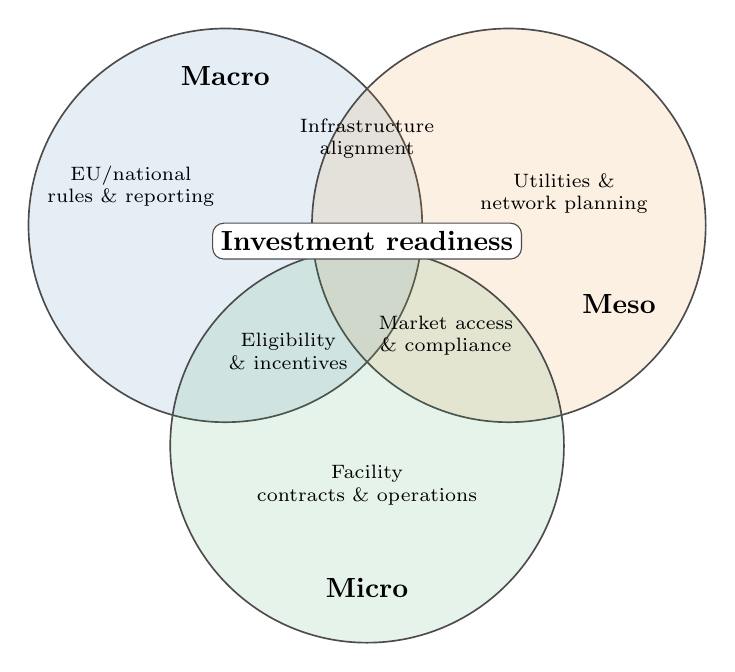
\begin{tikzpicture}

\def\r{2.5}

\definecolor{macrocol}{RGB}{52,120,180}
\definecolor{mesocol}{RGB}{230,140,40}
\definecolor{microcol}{RGB}{60,160,90}

\coordinate (A) at (0,0);
\coordinate (B) at (3.6,0);
\coordinate (C) at (1.8,-2.8);

% Lighter fills + softer outlines (print-friendly)
\draw[line width=0.6pt, draw=black!70, fill=macrocol, fill opacity=0.13] (A) circle (\r);
\draw[line width=0.6pt, draw=black!70, fill=mesocol,  fill opacity=0.13] (B) circle (\r);
\draw[line width=0.6pt, draw=black!70, fill=microcol, fill opacity=0.13] (C) circle (\r);

% --- Level labels (UNCHANGED size) ---
\node at (0,1.9) {\textbf{Macro}};
\node at (5.0,-1) {\textbf{Meso}};
\node at (1.8,-4.6) {\textbf{Micro}};

% --- Reduced internal texts ---
\node[align=center, font=\scriptsize] at (-1.2,0.5)
{EU/national\\rules \& reporting};

\node[align=center, font=\scriptsize] at (4.3,0.4)
{Utilities \&\\network planning};

\node[align=center, font=\scriptsize] at (1.8,-3.3)
{Facility\\contracts \& operations};

\node[align=center, font=\scriptsize] at (1.8,1.1)
{Infrastructure\\alignment};

\node[align=center, font=\scriptsize] at (0.8,-1.6)
{Eligibility\\\& incentives};

\node[align=center, font=\scriptsize] at (2.8,-1.4)
{Market access\\\& compliance};

% --- Central concept (keep prominent) ---
\node[draw=black!70, rounded corners, fill=white, inner sep=3pt]
at (1.8,-0.2)
{\textbf{Investment readiness}};

\end{tikzpicture}
\caption{Conceptual macro--meso--micro governance structure. Investment readiness emerges when regulatory signals, infrastructure feasibility, and project-level execution align. This structuring is adapted from the multi-level perspective in socio-technical transitions literature \cite{GEELS2020119894} to fit the data-center energy-integration context}
\label{fig:governance-venn}
\end{figure}


The macro--meso--micro framing used in Figure~\ref{fig:governance-venn} aligns with broader smart local energy systems perspectives that emphasize actor coordination and local context \cite{9}. Table~\ref{tab:governance-functions} summarizes typical governance functions that frequently appear in investment due diligence for integrated data-center projects. These functions are the operational bridge between policy intent and project execution: they determine whether integration assets can be financed, permitted, and operated with reliable revenue streams.

\begin{table}[t]
\centering
\footnotesize
\caption{Governance functions shaping investment readiness for system-integrated data centers.}
\label{tab:governance-functions}
\begin{tabularx}{\linewidth}{l X}
\toprule
Level & Typical functions relevant to investment readiness \\
\midrule
Macro (EU/national) & Climate targets, reporting requirements, carbon-price exposure, and market-design rules for flexibility that shape expected cash flows and eligibility for services \cite{7,8,15,16,Xu2023}. \\
Meso (regional/local) & Network planning and connection rights, congestion management, district-heating access and tariff design, land availability, zoning and permitting, and infrastructure sequencing that determine feasibility and timing \cite{21,22,23}. \\
Micro (project) & Heat-offtake and flexibility contracts, metering and telemetry, operational control, and risk allocation between operator, utility, and third parties \cite{23,12,13}. \\
\bottomrule
\end{tabularx}
\end{table}

The business implications of this cross-level misalignment are direct. A project that invests in integration assets can improve system outcomes and create long-term revenues, but still appear less efficient under conventional PUE reporting. This reduces coherence between profitability-driven investment decisions and KPI-centered reporting, particularly in service-active regimes where additional electricity use enables valuable system services. The analysis therefore motivates the need for a system-integrated performance indicator that preserves PUE comparability while internalizing external value.

The constraint set carried into the model reflects this business context. Demand is bounded by the IT workload profile, revenue timing risk is represented through lifecycle construction-delay accounting, and electricity-side constraints are captured through the hourly energy balance and the three-node DC-OPF network model. Heat-side constraints combine heat-exchanger capacity, heat-pump capacity, recoverable heat, pipe limits, and district-heating acceptance. Market-access and technical limits on flexibility are represented by installed controllable capacity, while storage is constrained by power, energy, and state-of-charge dynamics. Land constraints are represented by capacity-linked site requirements and annualized lease or opportunity costs. Together, these constraints translate macro policy, meso infrastructure, and micro finance into the optimization problem used to define and evaluate siPUE.

The following section introduces siPUE within this techno-economic framework.

\section{Methodological Contribution}
\label{sec:methodology}

This section formalizes the business logic described above and operationalizes it in a quantitative framework. The objective is to evaluate whether integration decisions that create system value are reflected coherently in the performance indicators used for reporting and investment screening. Standard practice relies on PUE, which remains the dominant benchmark in industry and in emerging reporting regimes \cite{Belady2008PUE,greengrid2014,ISO30134}. PUE is valuable as a simple internal-efficiency proxy, but it puts electricity used purely for cooling and electricity used to deliver externally valued services, such as heat export or flexibility provision, into the same overhead numerator. This creates the KPI gap described above: investments that improve system outcomes can appear worse on the headline metric even when the underlying economics improve.

The methodological contribution is a system-integrated companion indicator, siPUE, and a two-stage optimization framework that evaluates integration choices under uncertainty. siPUE extends the PUE structure by translating a separately accounted system-cost benefit into an energy-equivalent credit. This benefit covers avoided resource, transmission, peak, and carbon-damage cost, with private heat and flexibility revenue kept in the market objective. The metric is designed to be backward compatible with existing reporting (siPUE reduces to PUE when the system-cost credit is zero), while enabling forward compatibility with system-value creation.

The framework is explicitly business-oriented. It evaluates design decisions that require capital commitment (heat exchangers, heat pumps, flexibility capacity, batteries, and land use) together with operational decisions that respond to hourly market conditions (heat dispatch, reserve availability, storage operation). In the canonical configuration, the service-active cases also carry a fixed 15\% efficiency retrofit; the reported results treat this as a locked assumption outside the endogenous design variables. The objective function is a lifecycle market cost that explicitly prices electricity, carbon, capital, land, congestion, and service revenues, while also accounting for nodal import constraints and construction-delay effects. This structure mirrors the finance constraints described above: integration becomes bankable only when service revenues are credible and when policy or infrastructure constraints can be translated into predictable cash flows.

The evaluation protocol separates a metric-identity test from the fair headline comparison. The \emph{identity no-services} case fixes zero service capacities and zero efficiency investment, and is used only to verify that siPUE reduces to PUE when the system-benefit credit is zero. The \emph{fair services-disabled} comparator disables heat export, flexibility provision, and storage services, but keeps the same locked 15\% efficiency retrofit and the same carbon-cap, network, land, delay, demand, and operational assumptions as the service-active designs. The \emph{baseline} case is a fixed service-active design with incumbent levels of heat recovery, flexibility, battery, and the fixed efficiency retrofit. The \emph{robust} case is one shared design selected per archetype, over that archetype's own ten-scenario uncertainty set, via a min--max regret criterion, using scenario-specific perfect-foresight designs as upper-bound benchmarks. Baseline, robust, and scenario-perfect designs are evaluated against the same physical carbon cap as the fair services-disabled comparator. Because the original 5\% attributable-emissions cap is slightly below what the services-disabled efficient design can physically reach in most rows, the cap includes a services-disabled feasibility floor; this floor is applied in 39 of the 40 canonical rows and is reported in the output tables. PUE and siPUE are computed for all cases to test whether a system-integrated indicator provides a more coherent signal once integration assets are active.

\begin{figure}[H]
\centering
\footnotesize
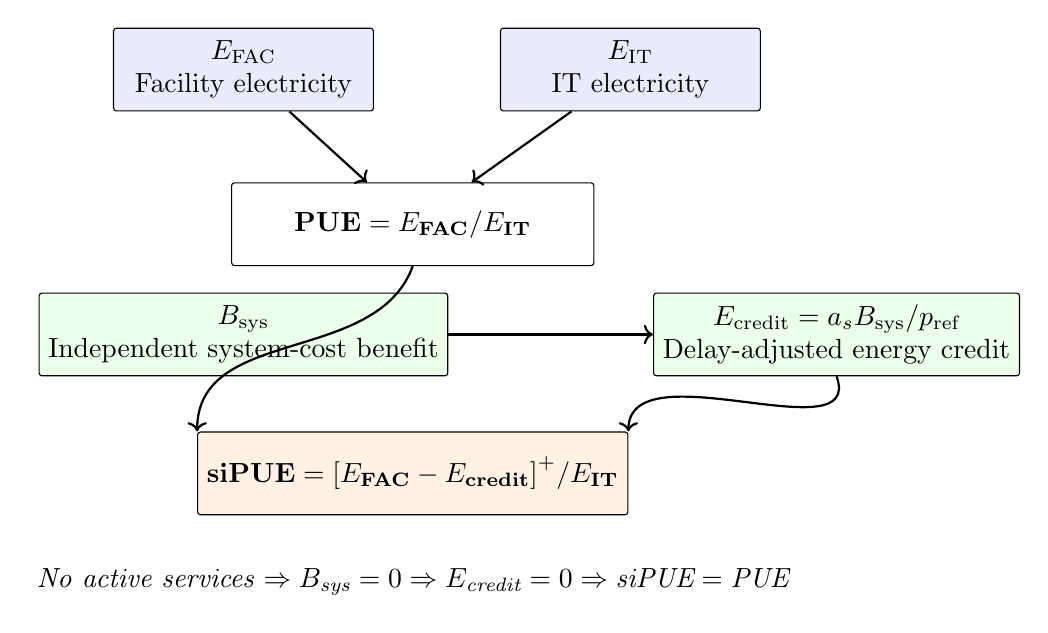
\begin{tikzpicture}[
box/.style={rectangle, draw, align=center, minimum width=3.3cm, minimum height=1.05cm, rounded corners=1pt},
sum/.style={rectangle, draw, align=center, minimum width=4.6cm, minimum height=1.05cm, rounded corners=1pt, font=\bfseries},
arrow/.style={->, thick}
]

\node[box, fill=blue!8] (efac) {$E_{\text{FAC}}$\\Facility electricity};
\node[box, fill=blue!8, right=1.6cm of efac] (eit) {$E_{\text{IT}}$\\IT electricity};
\node[sum, below=0.9cm of efac, xshift=2.15cm] (pue) {$\text{PUE}=E_{\text{FAC}}/E_{\text{IT}}$};
\draw[arrow] (efac) -- (pue);
\draw[arrow] (eit) -- (pue);

\node[box, fill=green!8, below=2.3cm of efac] (bsys) {$B_{\text{sys}}$\\Independent system-cost benefit};
\node[box, fill=green!8, right=2.6cm of bsys] (credit) {$E_{\text{credit}}=a_s B_{\text{sys}}/p_{\text{ref}}$\\Delay-adjusted energy credit};
\draw[arrow] (bsys) -- (credit);

\node[sum, fill=orange!10, below=2.1cm of pue] (sipue) {$\text{siPUE}=\left[E_{\text{FAC}}-E_{\text{credit}}\right]^{+}\!/E_{\text{IT}}$};
\draw[arrow] (pue.south) to[out=250,in=90] (sipue.north west);
\draw[arrow] (credit.south) to[out=290,in=90] (sipue.north east);

\node[below=0.55cm of sipue, align=center, font=\itshape] {No active services $\Rightarrow B_{\text{sys}}=0 \Rightarrow E_{\text{credit}}=0 \Rightarrow \text{siPUE}=\text{PUE}$};

\end{tikzpicture}
\caption{Metric logic for siPUE. PUE remains the internal energy ratio. siPUE subtracts a delay-adjusted, energy-equivalent credit for separately accounted system benefits. When no services are active, the credit is zero and siPUE equals PUE.}
\label{fig:sipue-metric-story}
\end{figure}

\begin{figure}[H]
\centering
\resizebox{0.98\linewidth}{!}{%
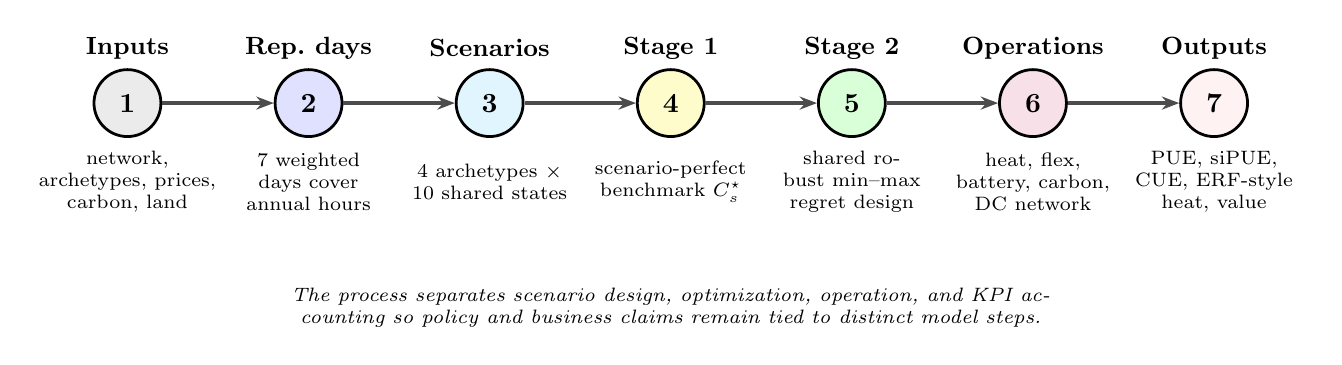
\begin{tikzpicture}[
x=1cm, y=1cm,
stagecircle/.style={circle, draw, minimum size=0.85cm, font=\bfseries, line width=1pt},
stagelabel/.style={font=\bfseries\small, align=center},
stagedetail/.style={font=\scriptsize, align=center, text width=2.3cm},
pipearrow/.style={-{Stealth[length=2.2mm]}, line width=1.2pt, color=black!70}
]

\node[stagelabel] (t1) at (0, 1.6) {Inputs};
\node[stagecircle, fill=black!8] (c1) at (0, 0.9) {1};
\node[stagedetail] (d1) at (0, -0.1) {network, archetypes, prices, carbon, land};

\node[stagelabel] (t2) at (2.3, 1.6) {Rep.\ days};
\node[stagecircle, fill=blue!12] (c2) at (2.3, 0.9) {2};
\node[stagedetail] (d2) at (2.3, -0.1) {7 weighted days cover annual hours};

\node[stagelabel] (t3) at (4.6, 1.6) {Scenarios};
\node[stagecircle, fill=cyan!12] (c3) at (4.6, 0.9) {3};
\node[stagedetail] (d3) at (4.6, -0.1) {4 archetypes $\times$ 10 shared states};

\node[stagelabel] (t4) at (6.9, 1.6) {Stage 1};
\node[stagecircle, fill=yellow!20] (c4) at (6.9, 0.9) {4};
\node[stagedetail] (d4) at (6.9, -0.1) {scenario-perfect benchmark $C_s^{\star}$};

\node[stagelabel] (t5) at (9.2, 1.6) {Stage 2};
\node[stagecircle, fill=green!15] (c5) at (9.2, 0.9) {5};
\node[stagedetail] (d5) at (9.2, -0.1) {shared robust min--max regret design};

\node[stagelabel] (t6) at (11.5, 1.6) {Operations};
\node[stagecircle, fill=purple!12] (c6) at (11.5, 0.9) {6};
\node[stagedetail] (d6) at (11.5, -0.1) {heat, flex, battery, carbon, DC network};

\node[stagelabel] (t7) at (13.8, 1.6) {Outputs};
\node[stagecircle, fill=pink!20] (c7) at (13.8, 0.9) {7};
\node[stagedetail] (d7) at (13.8, -0.1) {PUE, siPUE, CUE, ERF-style heat, value};

\draw[pipearrow] (c1) -- (c2);
\draw[pipearrow] (c2) -- (c3);
\draw[pipearrow] (c3) -- (c4);
\draw[pipearrow] (c4) -- (c5);
\draw[pipearrow] (c5) -- (c6);
\draw[pipearrow] (c6) -- (c7);

\node[font=\scriptsize\itshape, align=center, text width=13cm] at (6.9, -1.7) {The process separates scenario design, optimization, operation, and KPI accounting so policy and business claims remain tied to distinct model steps.};

\end{tikzpicture}
}
\caption{Model pipeline from inputs and scenarios to robust design, KPI outputs, and internal diagnostics.}
\label{fig:model-pipeline}
\end{figure}

\subsection{Definition and interpretation of siPUE}

PUE is defined as
\begin{equation}
\text{PUE} = \frac{E_{\text{FAC}}}{E_{\text{IT}}},
\end{equation}
where $E_{\text{FAC}}$ is modeled facility electricity and $E_{\text{IT}}$ is delivered IT electricity. The proposed siPUE keeps this denominator and adjusts only the numerator. It is a PUE-compatible companion indicator that converts separately accounted local-system benefits, including heat, flexibility, peak, carbon damage, and delay, into an energy-equivalent numerator credit. Let superscript $0$ denote the fair services-disabled comparator and $d$ denote a service-active design. The independent system-accounting ledger is
\begin{equation}
C_{\text{ind}}^d =
C_{\text{el}}^d
+ C_{\text{trans}}^d
+ C_{\text{peak}}^d
+ C_{\text{CO2,dam}}^d
- V_{\text{heat}}^d
- V_{\text{flex}}^d ,
\label{eq:independent-cost-ledger}
\end{equation}
where $C_{\text{el}}$ is electricity resource cost, $C_{\text{trans}}$ is transmission or network cost, $C_{\text{peak}}$ is the independent peak-capacity cost, $C_{\text{CO2,dam}}$ is the carbon-damage ledger, and $V_{\text{heat}}$ and $V_{\text{flex}}$ are separately accounted avoided heat and flexibility costs. The net system benefit credited by siPUE is the counterfactual reduction in this independent accounting ledger:
\begin{equation}
B_{\text{sys}}^d =
C_{\text{ind}}^0 - C_{\text{ind}}^d .
\label{eq:system-benefit}
\end{equation}
Equivalently, positive terms in $B_{\text{sys}}$ are avoided independent system costs, while negative terms are additional system burdens from the service-active design. No component is truncated before aggregation. A design with net negative $B_{\text{sys}}$ therefore receives a negative energy credit and its siPUE increases relative to PUE; the outer $[\cdot]^+$ operator in Eq.~\ref{eq:sipue} only prevents the adjusted numerator from becoming negative when net benefits are very large.

\begin{table}[H]
\centering
\small
\caption{Accounting boundary for the siPUE system-benefit term.}
\label{tab:sipue-boundary}
\begin{tabularx}{\linewidth}{X X}
\toprule
Included in $B_{\text{sys}}$ & Excluded from $B_{\text{sys}}$ \\
\midrule
Electricity resource-cost changes, transmission or network-cost changes, independent peak-capacity effects, carbon-damage changes, avoided heat-system cost, and avoided flexibility-system cost. & Private heat and flexibility revenues, IT service revenue, ETS or carbon-market payments, capex, land lease or opportunity cost, private demand charges, taxes, subsidies, and financing terms. \\
\bottomrule
\end{tabularx}
\end{table}

This boundary keeps private settlement and public system value separate. Private heat and flexibility revenues appear in the market-cost objective, while siPUE credits only independent system benefit. Conversely, carbon-market payments are kept in the private market ledger, while carbon damage enters only the independent system ledger. This separation avoids counting a private payment as a public system benefit or counting the same carbon effect twice.

\begin{table}[H]
\centering
\small
\caption{Dimensional and temporal basis of the siPUE terms.}
\label{tab:sipue-units}
\begin{tabularx}{\linewidth}{L{2.7cm} L{2.4cm} X L{2.2cm}}
\toprule
Term & Unit & Temporal basis & Discounted? \\
\midrule
$E_{\text{FAC}}$ & MWh/year & Representative modeled operating year. & No \\
$E_{\text{IT}}$ & MWh/year & Same representative modeled operating year. & No \\
$B_{\text{sys}}$ & EUR/year & Annual system-benefit difference between the fair services-disabled comparator and design $d$. & No \\
$p_{\text{ref}}$ & EUR/MWh & Frozen base-case reference price used only for unit conversion. & No \\
$a_s$ & dimensionless & Lifecycle availability factor applied once to represent delayed useful benefit. & No \\
\bottomrule
\end{tabularx}
\end{table}

The delay-adjusted energy credit is
\begin{equation}
E_{\text{credit}} =
a_s \frac{B_{\text{sys}}}{p_{\text{ref}}},
\label{eq:sipue-credit}
\end{equation}
where $p_{\text{ref}}$ is the calibrated electricity reference price in EUR/MWh and $a_s \in [0,1]$ is the lifecycle availability factor after construction delay. The reference price functions only as a unit converter. In the canonical run it is fixed before optimization at 56.63~EUR/MWh, based on the no-services electricity-resource marginal cost at the data-center node. ETS payments and carbon damage are excluded from $p_{\text{ref}}$ because those terms are already handled in separate ledgers. Freezing $p_{\text{ref}}$ across all designs and uncertainty states prevents the metric from improving simply because the conversion factor changes.

siPUE is
\begin{equation}
\text{siPUE} =
\frac{\left[E_{\text{FAC}} - E_{\text{credit}}\right]^+}{E_{\text{IT}}},
\label{eq:sipue}
\end{equation}
with $[z]^+=\max(0,z)$. Internal property checks are run before interpretation: nonnegativity (checked separately for the identity no-services, fair services-disabled, baseline, and robust cases), the no-services identity, delay monotonicity, carbon-ledger separation, canonical scenario count, scale normalization, benefit monotonicity, delay behavior, and reference-price monotonicity. These are verification checks of the metric construction, not external validation against observed projects. The property table (Figure~\ref{fig:property-checks}) satisfies all checks.

\subsection{Reference-price sensitivity and anti-gaming rule}
\label{sec:pref-sensitivity}

The reference price is the main conversion choice in siPUE, so it is treated as a first-order sensitivity. Holding design and operation fixed, a multiplier $k$ gives
\begin{equation}
\text{siPUE}(k) =
\frac{\left[E_{\text{FAC}} - a_s B_{\text{sys}} /(k p_{\text{ref}})\right]^+}{E_{\text{IT}}}.
\label{eq:sipue-pref-sensitivity}
\end{equation}

The anti-gaming rule is that $p_{\text{ref}}$ must be selected before the service-active design is evaluated. In this study it is the frozen no-services electricity-resource marginal cost at the data-center node. It is fixed ex ante by the analyst, before observing service-active outcomes, and remains constant across designs and uncertainty states. ETS payments and carbon damage are excluded from $p_{\text{ref}}$ because those effects already enter separate ledgers. The sensitivity in Table~\ref{tab:pref-sensitivity} recomputes only Eq.~\ref{eq:sipue-pref-sensitivity}; dispatch, heat delivery, emissions, PUE, and the sign of $B_{\text{sys}}$ are unchanged.

\begin{table}[tbp]
\centering
\small
\caption{Reference-price sensitivity for the canonical robust rows. Dispatch and ledgers are held fixed; only the value-to-energy conversion factor changes. Average siPUE uses IT-energy weights across archetypes.}
\label{tab:pref-sensitivity}
\begin{tabularx}{\linewidth}{L{3.0cm} Y r}
\toprule
Reference-price case & Interpretation & Average siPUE \\
\midrule
$0.5p_{\text{ref}}$ & Low conversion price; stronger energy credit & 0.961 \\
$1.0p_{\text{ref}}$ & Canonical frozen reference price & 1.152 \\
$1.5p_{\text{ref}}$ & High conversion price; weaker energy credit & 1.216 \\
\bottomrule
\end{tabularx}
\end{table}

This sensitivity is intentionally large enough to report: the reference price affects the magnitude of the siPUE credit, even though the underlying physical and monetary ledgers remain unchanged. For that reason, siPUE should always be reported with the reference-price rule and a sensitivity band.

siPUE is a system-adjusted performance indicator with a different interpretation from thermodynamic efficiency. It is designed as a companion KPI beside PUE. For operators and investors, it gives a KPI view of external value that can be read next to PUE. For policy users, it gives a way to discuss heat recovery and flexibility without treating every MWh of additional facility electricity as waste.

\subsection{Two-stage design model}

Let $s \in \mathcal{S}$ index the shared uncertainty states, $x$ denote design variables, and $y_s$ denote hourly operational variables. Stage~1 solves a scenario-perfect benchmark:
\begin{equation}
C_s^{\star} = \min_{x,y_s} C_s(x,y_s),
\label{eq:stage-one}
\end{equation}
where $C_s$ is lifecycle market cost for scenario $s$. Stage~2 chooses one shared design $\hat{x}$ per archetype, applying the minimax-regret criterion discussed in Section~\ref{sec:related} \cite{savage1951theory,MR-1626-RPC}. The ten shared states are left unweighted by probabilities; each archetype is solved independently over its own ten-scenario group. The resulting canonical analysis contains four shared designs, one per archetype, with no single design shared across all 40 rows. Regret is computed against the scenario-perfect benchmark and normalized by each scenario's present-value-discounted lifetime IT energy $E_{\text{IT},s}^{\text{PV}}$, so it is reported in EUR/MWh IT:
\begin{equation}
R_s(\hat{x}) =
\frac{C_s(\hat{x},y_s)-C_s^{\star}}{\max(\epsilon, E_{\text{IT},s}^{\text{PV}})}.
\label{eq:normalised-regret}
\end{equation}
The robust design is selected in two passes: the first minimizes the worst normalized regret across scenarios, giving $Z^{\star}$ from Eq.~\ref{eq:normalised-regret}; the second fixes $Z \le Z^{\star}(1+\tau)$ and, within that near-worst-case band, minimizes mean lifecycle cost across scenarios. This is a lexicographic tie-break \cite{Miettinen1999,Ehrgott2005,MarlerArora2004}. In the canonical run $\tau = 10^{-7}$, so this tie-break resolves numerically degenerate ties at the worst-case-regret optimum while preserving worst-case regret to material precision. The canonical results report the identity no-services case, the fair services-disabled comparator, the fixed baseline design, and the robust shared design. Scenario-perfect solutions serve as planning benchmarks and validation references.

The implementation can enumerate discrete efficiency-reduction levels, but the canonical run fixes the efficiency reduction at 0.15 in the fair services-disabled, baseline, robust, and scenario-perfect cases. The optimized capacity choices reported below are therefore heat-exchanger capacity, heat-pump capacity, flexibility capacity, battery energy and power capacity, and associated land use. The identity no-services case keeps both service capacity and efficiency reduction at zero.

\begin{figure}[H]
\centering
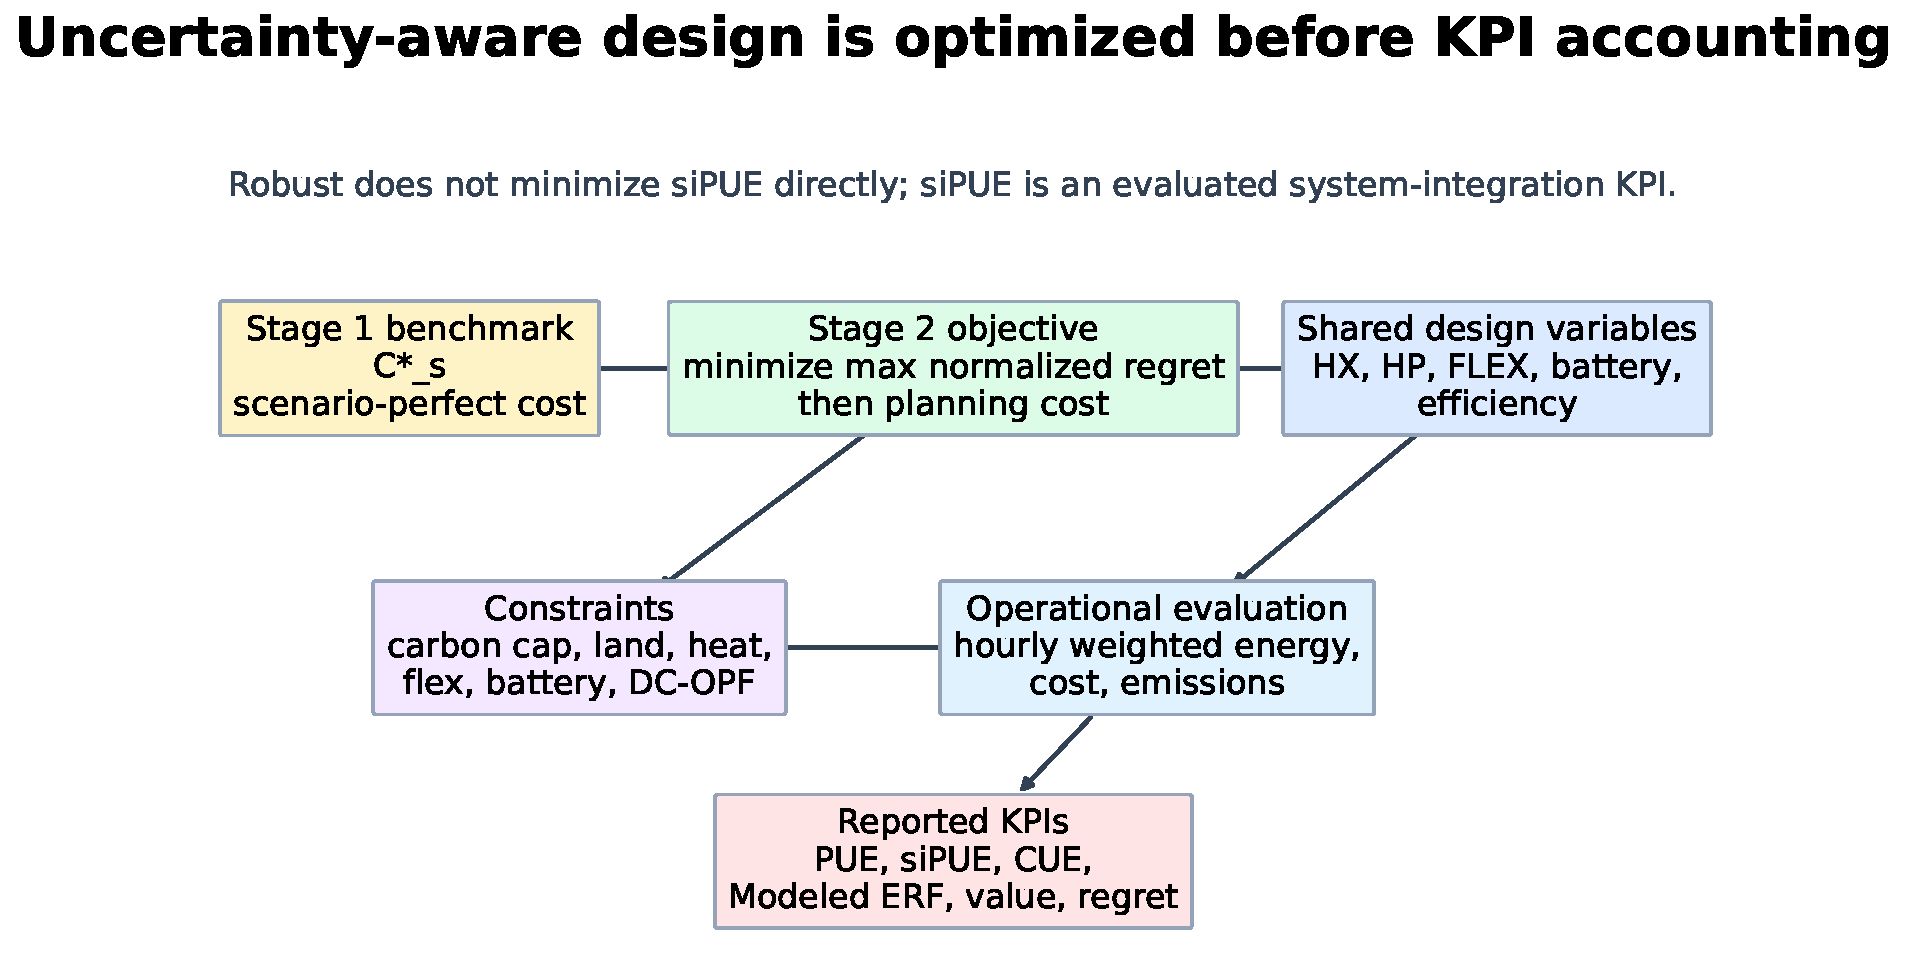
\includegraphics[width=0.95\linewidth]{fig_05_optimization_formulation_map.pdf}
\caption{Optimization map linking design variables, scenario-perfect benchmarks, normalized regret, and physical constraints.}
\label{fig:optimization-map}
\end{figure}

\subsection{Operational constraints and ledgers}

Hourly operation is represented as a linear program. The facility energy balance links grid import, battery charging and discharging, IT load, cooling overhead, and heat-pump electricity. Heat export is bounded by heat-exchanger capacity, heat-pump capacity, recoverable heat, pipe limits, and district-heating acceptance. Flexibility is modeled as an availability or reserve-capacity service, consistent with reserve products whose settlement depends on capacity availability and telemetry, with routine energy delivery outside the settlement basis \cite{13,Takci2025,Crozier2025}. The reserve variables for controllable load and battery headroom earn private flexibility revenue and, for controllable load, an avoided system-cost credit; the nodal power balance includes actual facility load and parasitic service overhead. Deliverability is represented through headroom constraints on IT load, installed controllable capacity, unused battery inverter capacity, stored energy above the UPS reserve, and parasitic service overhead. Scarcity-event activation is outside the current validation scope. Battery operation follows state-of-charge dynamics with charge and discharge limits.

The electricity system is represented by a stylized three-node DC-OPF. Thermal generation, renewable availability, line capacities, and nodal settlement prices determine the cost of supplying the data center and the wider network.

Carbon is kept in separate ledgers: market carbon cost enters the private market ledger, and carbon damage enters the independent system-cost ledger. They are reported together while remaining separate from private-credit claims. Land is modeled as lease or opportunity-cost accounting tied to core facility, cooling, heat, flexibility, and battery footprints. This stylized constraint supports design comparison; physical siting analysis remains outside the model scope.

\subsection{Data and scenario design}

The model uses a calibrated three-node hourly time series with 8,760 sequential hours. The annual run is compressed into seven representative days. Hourly weights sum to 8,760 and day weights sum to 365, so operating quantities are annualized once. Fixed annual terms, such as capex, demand charges, and land lease cost, enter once outside the representative-day weighting.

The scenario set has four archetypes and ten shared uncertainty states, giving 40 canonical rows. The archetypes are AI/HPC, hyperscale cloud, colocation, and enterprise/edge. Each uncertainty state changes service prices, heat conditions, construction delay, carbon caps, and related operating conditions using predefined scenario construction. The physical carbon cap is common to the fair services-disabled, baseline, robust, and scenario-perfect cases within each row. The archetype base recoverable-heat fractions are 0.20--0.50, informed by data-center heat-reuse literature and adjusted downward where archetype-specific evidence is weak \cite{10,11,Yuan2025,Hao2025}. State multipliers then represent local heat-network opportunity and raise some effective LP inputs above the base range; in the canonical rows the effective recoverable-heat fraction spans 0.17--0.575, with the largest values occurring for AI/HPC and hyperscale in favorable heat states. The design and KPI outputs are normalized by IT energy or IT capacity where appropriate, so capacity comparisons are interpretable across archetypes.

\begin{table}[H]
\centering
\small
\caption{Canonical scenario structure used in the model evaluation.}
\label{tab:canonical-scenario-structure}
\begin{tabularx}{\linewidth}{L{3.1cm} r Y}
\toprule
Dimension & Count & Role in the model \\
\midrule
Archetypes & 4 & AI/HPC, hyperscale cloud, colocation, enterprise/edge \\
Shared uncertainty states & 10 & Heat, flexibility, carbon-cap, delay, and service conditions \\
Canonical rows & 40 & One row for each archetype and uncertainty-state pair \\
Canonical design cases & 4 & identity no-services, fair services-disabled, baseline, robust \\
Representative days & 7 & Weighted annual operating approximation \\
\bottomrule
\end{tabularx}
\end{table}

\begin{figure}[H]
\centering
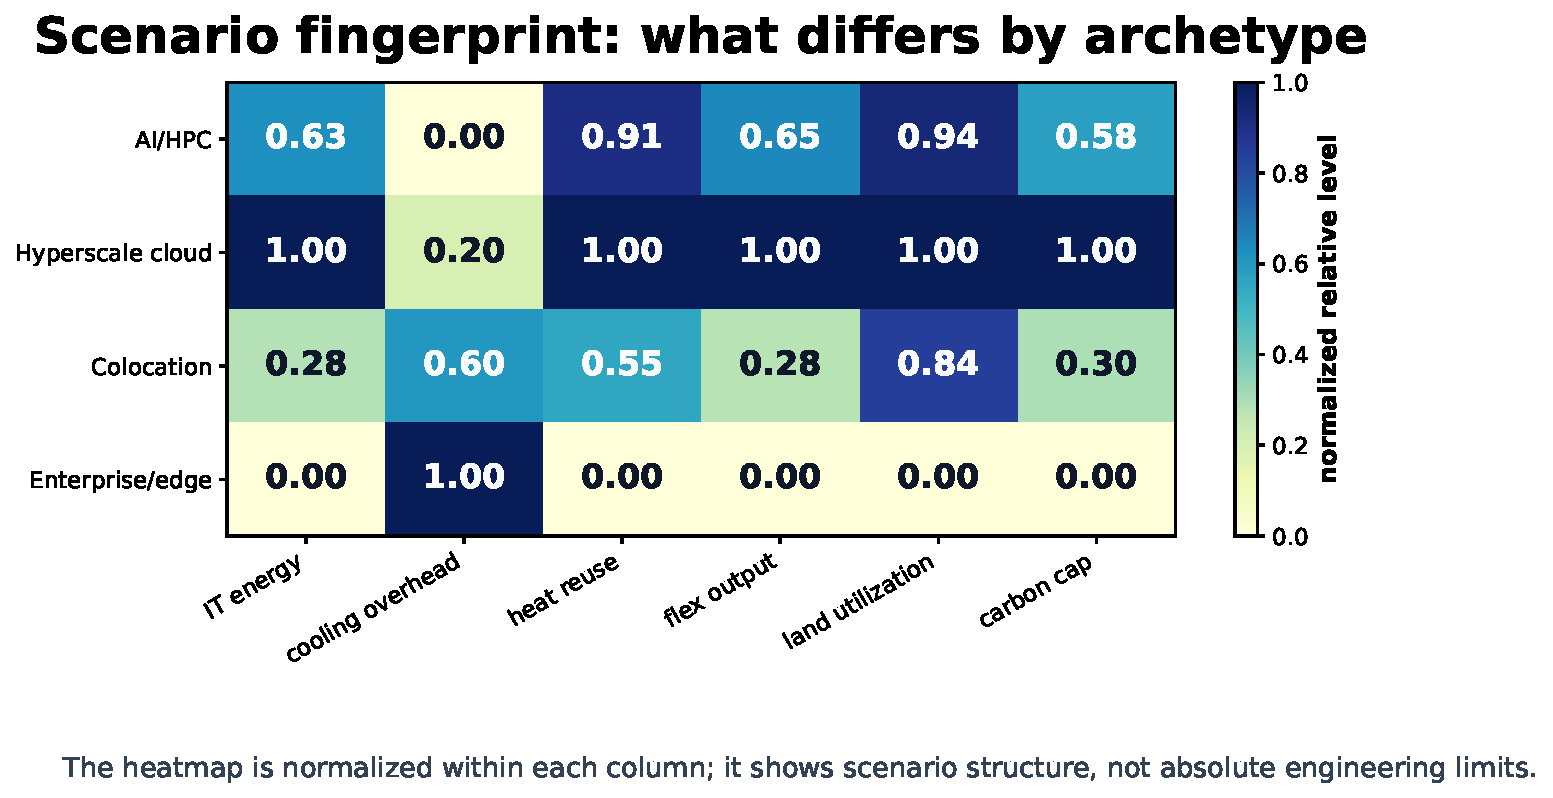
\includegraphics[width=0.92\linewidth]{fig_06_input_scenario_fingerprint.pdf}
\caption{Input scenario fingerprint, normalized within each column to show relative scenario structure.}
\label{fig:scenario-fingerprint}
\end{figure}

\begin{figure}[H]
\centering
\begin{subfigure}{0.48\linewidth}
\centering
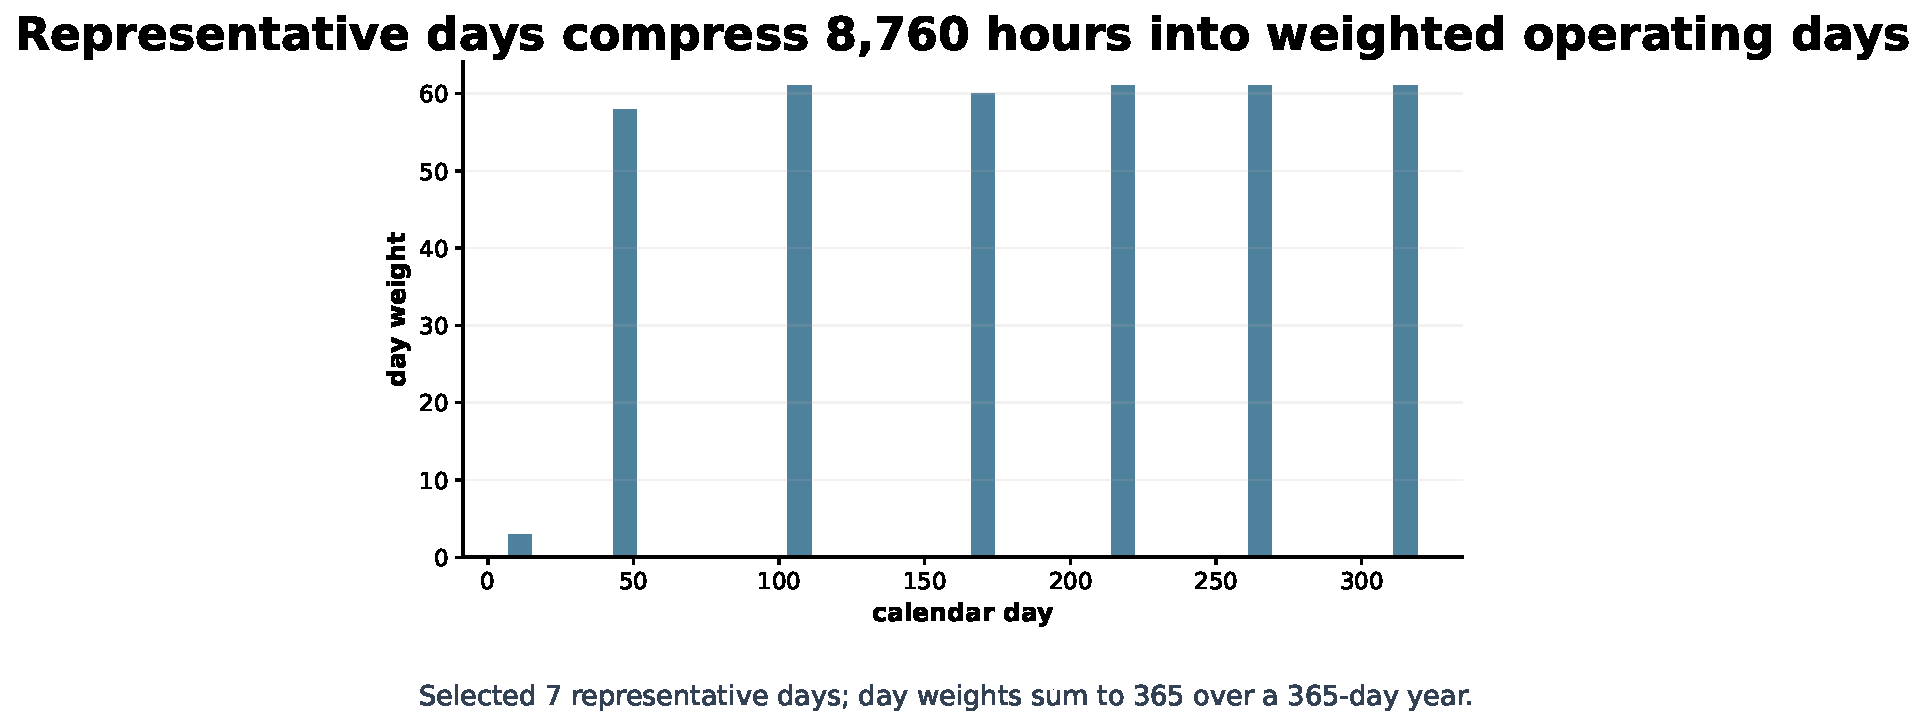
\includegraphics[width=\linewidth]{fig_07a_representative_day_weights.pdf}
\caption{Selected representative days and weights.}
\end{subfigure}
\hfill
\begin{subfigure}{0.48\linewidth}
\centering
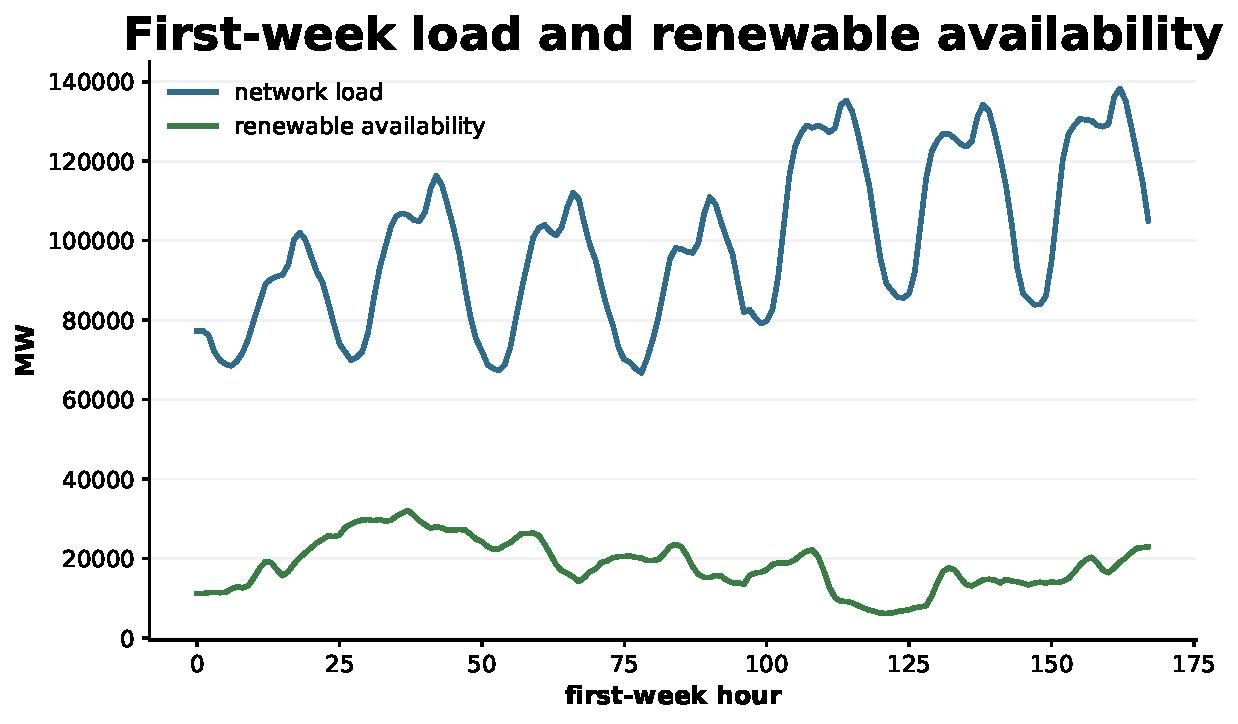
\includegraphics[width=\linewidth]{fig_07b_representative_day_load_trace.pdf}
\caption{First-week load and renewable profiles.}
\end{subfigure}
\caption{Representative-day compression and hourly system context.}
\label{fig:representative-days}
\end{figure}

\begin{figure}[H]
\centering
\begin{subfigure}{0.32\linewidth}
\centering
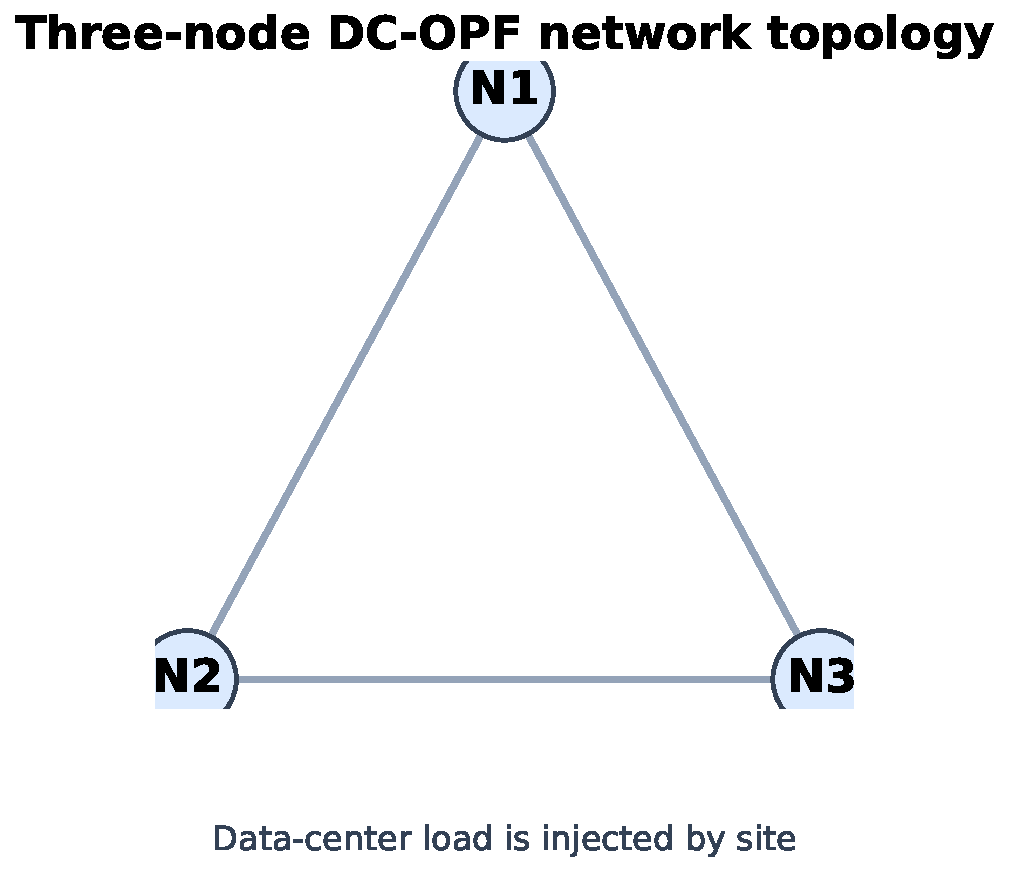
\includegraphics[width=\linewidth]{fig_08a_network_topology.pdf}
\caption{Network topology.}
\end{subfigure}
\hfill
\begin{subfigure}{0.32\linewidth}
\centering
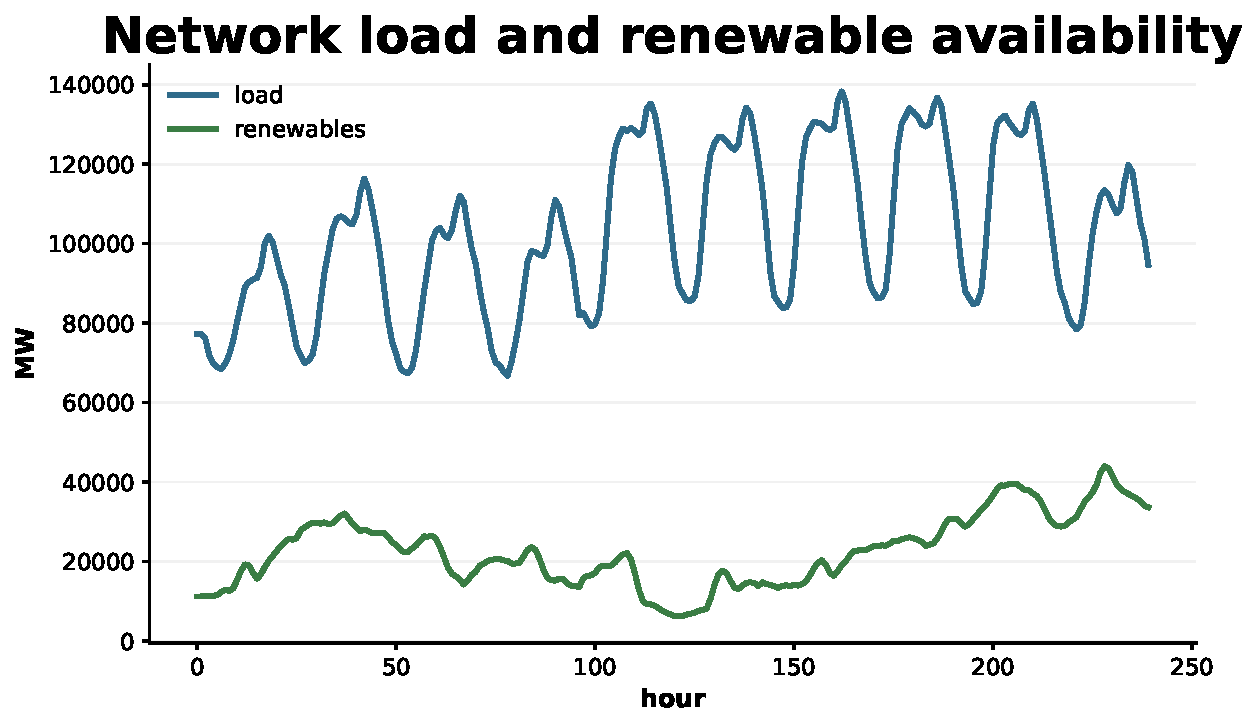
\includegraphics[width=\linewidth]{fig_08b_load_and_renewables.pdf}
\caption{Load and renewables.}
\end{subfigure}
\hfill
\begin{subfigure}{0.32\linewidth}
\centering
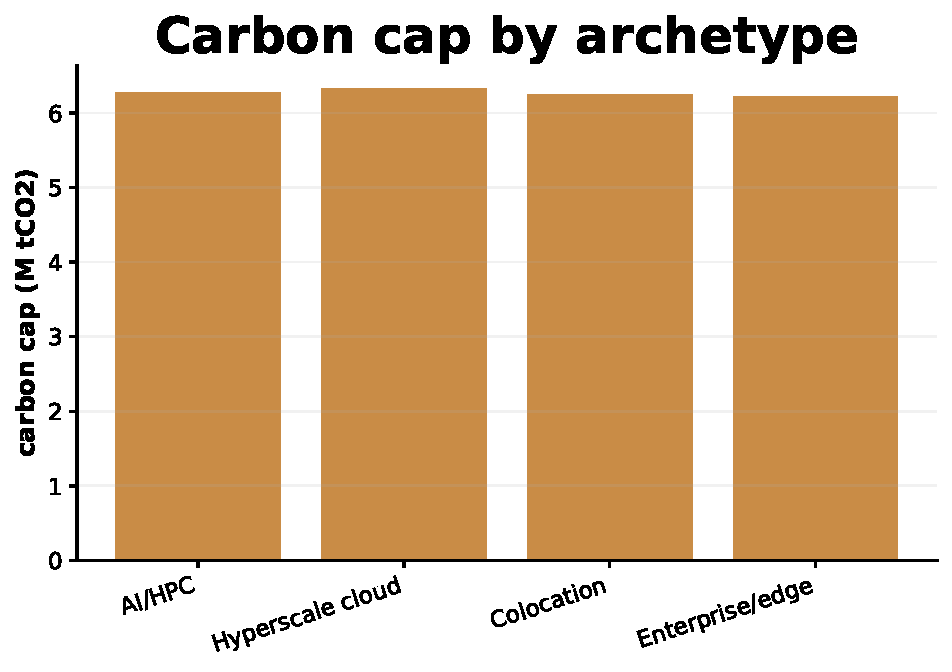
\includegraphics[width=\linewidth]{fig_08c_carbon_cap_by_archetype.pdf}
\caption{Carbon-cap context.}
\end{subfigure}
\caption{Stylized electricity-network and carbon context used by the operational model.}
\label{fig:network-context}
\end{figure}

\section{Results and Discussion}
\label{sec:results}

The results are organized around one claim and then the diagnostics needed to qualify it. The metric benchmark first shows how PUE and siPUE move when service assets are introduced. The credit decomposition and portfolio figures then explain why the movement occurs. The validation, sensitivity, and face-validity sections test whether that interpretation is internally consistent, robust to important assumptions, and plausible next to published benchmarks \cite{UptimeInstitute2024Survey,EUSmartCities2024Mantsala}.

\subsection{PUE and siPUE move differently}

Table~\ref{tab:kpi-summary} reports average modeled metrics from the canonical output, weighted by each archetype's annual IT energy: each archetype's ten rows are scaled by its installed IT capacity (8--60~MW across the four archetypes), so an archetype with more IT energy contributes proportionally more to the average. The identity no-services case gives the required metric identity: PUE and siPUE are both 1.196 on average. The fair services-disabled comparator, with the same locked efficiency retrofit and the same physical carbon-cap treatment as the service-active cases, has PUE and siPUE of 1.167. This is the headline reference for the service-active comparison.

Against that fair comparator, the baseline design raises average PUE to 1.238, a 0.071 increase, while lowering average siPUE to 1.139, a 0.028 decrease. Baseline earns 5.603~EUR/MWh IT of delay-adjusted system benefit, equal to an energy-equivalent credit of about 0.099~MWh/MWh IT at the frozen 56.63~EUR/MWh reference price, or about 1.40 times its facility-energy burden. The robust design raises PUE further, to 1.343, a 0.176 increase, while lowering siPUE to 1.152, a 0.015 decrease. It earns a larger absolute benefit than baseline, 10.825~EUR/MWh IT, but its credit-to-burden ratio is smaller, about 1.08. The result is therefore not that robust is ``better according to siPUE'' than baseline; baseline has the lower average siPUE. The robust design creates more absolute system value, but with a lower benefit-to-facility-burden ratio, consistent with diminishing marginal system value as integration intensity scales.

The credit is an economic conversion, separate from physical energy savings; it is the separately priced local-system value created by service delivery. PUE therefore records the extra electricity, while siPUE records that electricity net of the explicit system-value credit, moving above or below PUE depending on whether the credit tracks the burden it is meant to offset. The carbon-exclusion diagnostic below provides the most direct stress test of this result: the average siPUE improvement is no longer present when carbon damage is removed from the accounting ledger.

\begin{table}[H]
\centering
\scriptsize
\setlength{\tabcolsep}{3pt}
\caption{Compact metric benchmark across the 40 canonical rows, weighted by each archetype's annual IT energy. Carbon, heat, and emissions are kept as separate ledgers with their own labels.}
\label{tab:kpi-summary}
\begin{tabularx}{\linewidth}{L{3.05cm} >{\raggedleft\arraybackslash}X >{\raggedleft\arraybackslash}X >{\raggedleft\arraybackslash}X >{\raggedleft\arraybackslash}X >{\raggedleft\arraybackslash}X}
\toprule
Design case & PUE & siPUE & Post-constr. siPUE & System benefit (EUR/MWh IT) & Benefit excl. carbon (EUR/MWh IT) \\
\midrule
Identity no-services & 1.196 & 1.196 & 1.196 & 0.000 & 0.000 \\
Fair services-disabled & 1.167 & 1.167 & 1.167 & 0.000 & 0.000 \\
Baseline & 1.238 & 1.139 & 1.135 & 5.603 & 3.433 \\
Robust & 1.343 & 1.152 & 1.145 & 10.825 & 5.161 \\
\bottomrule
\end{tabularx}
\end{table}

Baseline, the fixed service-active design with lower integration intensity, has the lowest average siPUE, but it also has much lower heat-reuse intensity than the robust design. The robust case is selected for cost-regret robustness across the uncertainty set, with minimum siPUE outside the selection criterion. The comparison therefore separates two questions: which design is robust under market and system uncertainty, and whether the resulting service-active design is evaluated fairly by PUE alone.

The scenario-level result remains heterogeneous under this fair-comparator framing. siPUE is lower than the fair services-disabled comparator in 36 of 40 baseline rows and 23 of 40 robust rows. PUE is higher than the fair comparator in all baseline and robust rows. Figure~\ref{fig:tradeoff-compass} shows the paired movement within each row. Each arrow starts from the baseline design and ends at the robust design, with both coordinates measured as changes relative to the constrained services-disabled comparator. The remaining robust rows are concentrated where the additional system-value credit is small relative to the facility-energy burden it is paying for.

\begin{figure}[H]
\centering
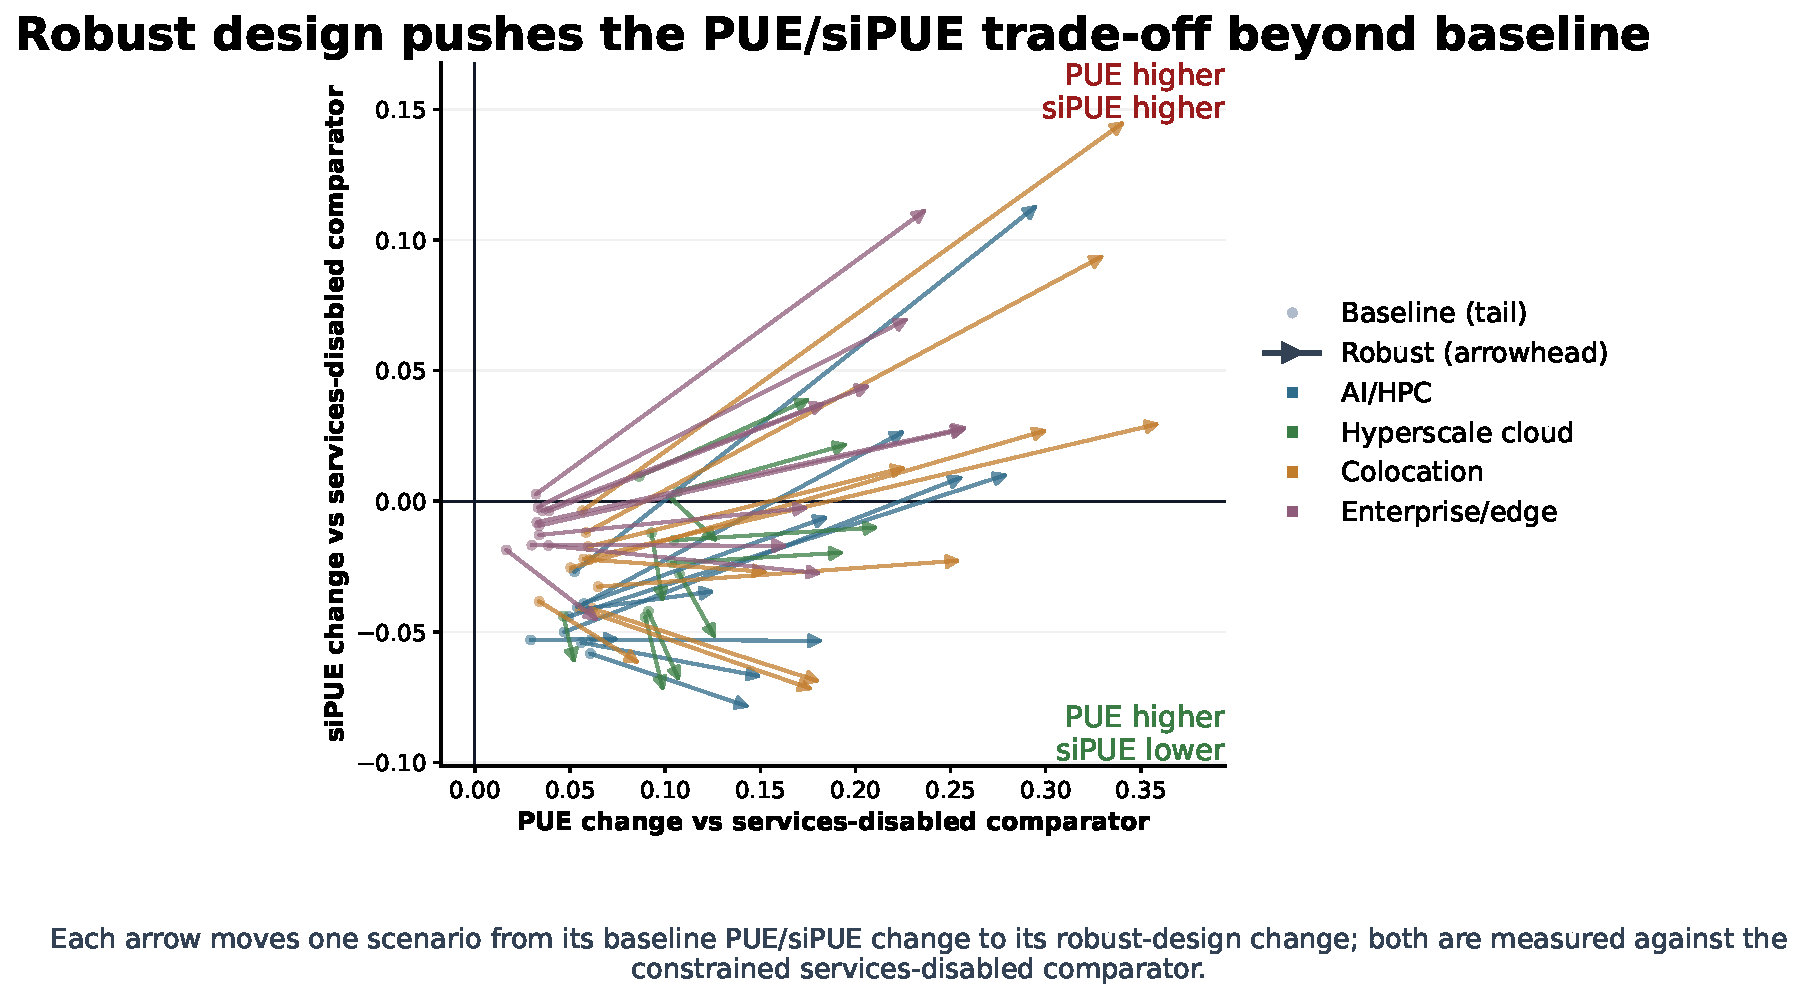
\includegraphics[width=0.92\linewidth]{fig_03_pue_sipue_tradeoff_compass.pdf}
\caption{PUE and siPUE tradeoff compass. Each arrow moves one scenario from the baseline design to the robust design, with both metrics measured as change relative to the constrained services-disabled comparator.}
\label{fig:tradeoff-compass}
\end{figure}

\subsection{Credit decomposition}

Table~\ref{tab:credit-ablation} decomposes the robust siPUE credit into the independent accounting-ledger components that create or reduce local-system value. Positive entries reduce siPUE because they lower independent system cost relative to the fair services-disabled comparator. Negative entries raise siPUE because they are additional system burdens from the service-active design. The robust design creates large heat, flexibility, and carbon-damage benefits, but those benefits are partly offset by additional electricity-resource, peak-capacity, and transmission burdens. Construction delay then weakens the credit before it enters the siPUE numerator.

\begin{table}[tbp]
\centering
\small
\caption{Component ablation of the robust siPUE credit across the 40 canonical rows, weighted by each archetype's annual IT energy. Values are EUR/MWh IT. Components above the delay row are before lifecycle delay; the final row is the delay-adjusted benefit credited by siPUE.}
\label{tab:credit-ablation}
\begin{tabularx}{\linewidth}{L{3.2cm} r Y}
\toprule
Component & Contribution & Interpretation \\
\midrule
Heat system value & 10.953 & Avoided independent heat-system cost \\
Flexibility system value & 3.799 & Avoided independent flexibility cost \\
Carbon damage & 5.864 & Avoided carbon-damage ledger cost \\
Peak capacity & -1.182 & Additional independent peak-capacity burden \\
Electricity resource cost & -7.834 & Additional power-system resource burden \\
Transmission / network cost & -0.371 & Additional network-flow burden \\
\midrule
Undelayed system benefit & 11.231 & Net benefit before delay adjustment \\
Construction-delay adjustment & -0.405 & Lost credit from delayed availability \\
\midrule
Delay-adjusted system benefit & 10.825 & Benefit entering the siPUE numerator \\
\bottomrule
\end{tabularx}
\end{table}

The ablation explains the value channel omitted by PUE. The service-active design uses substantially more facility electricity, so PUE rises. siPUE treats that burden explicitly and subtracts only the separately accounted system-cost benefit, converted through the frozen reference price. The reported score therefore shows both sides of the trade: higher facility energy and the heat, flexibility, carbon-damage, peak, and delay value created outside the facility boundary. Carbon damage is material: excluding it raises the IT-weighted robust siPUE from 1.152 to 1.252, above the fair services-disabled comparator's 1.167, and only 4 of 40 robust rows remain below the comparator without the carbon-damage term. The metric result should therefore be read as conditional on the stated social-carbon valuation, not as carbon-valuation-independent evidence.

\subsection{Design portfolios and system value}

The robust design changes the technology portfolio. Figure~\ref{fig:portfolio} shows the capacity intensity of heat recovery, heat pumps, flexibility, and batteries by archetype. Figure~\ref{fig:value-flow} decomposes the resulting system value. These figures keep the economic story visible: higher facility energy can be a cost of delivering heat and flexibility services, but the benefit depends on the local price, heat, land, and delay conditions.

\begin{figure}[H]
\centering
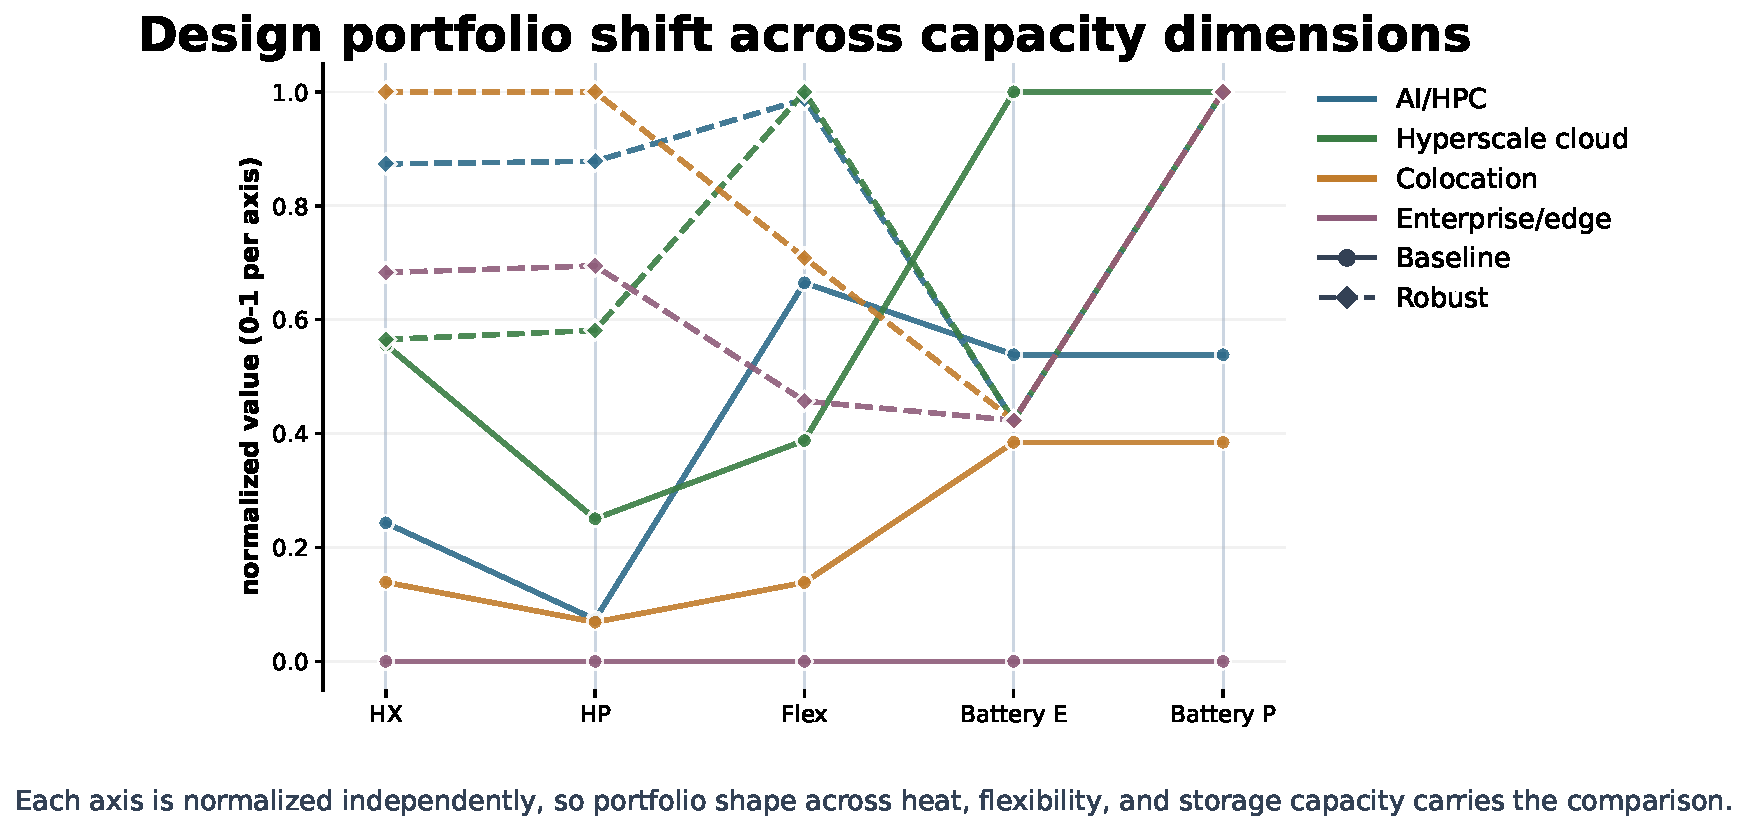
\includegraphics[width=0.95\linewidth]{fig_09_design_portfolio_parallel.pdf}
\caption{Baseline and robust design portfolios by archetype, normalized per MW IT.}
\label{fig:portfolio}
\end{figure}

\begin{figure}[H]
\centering
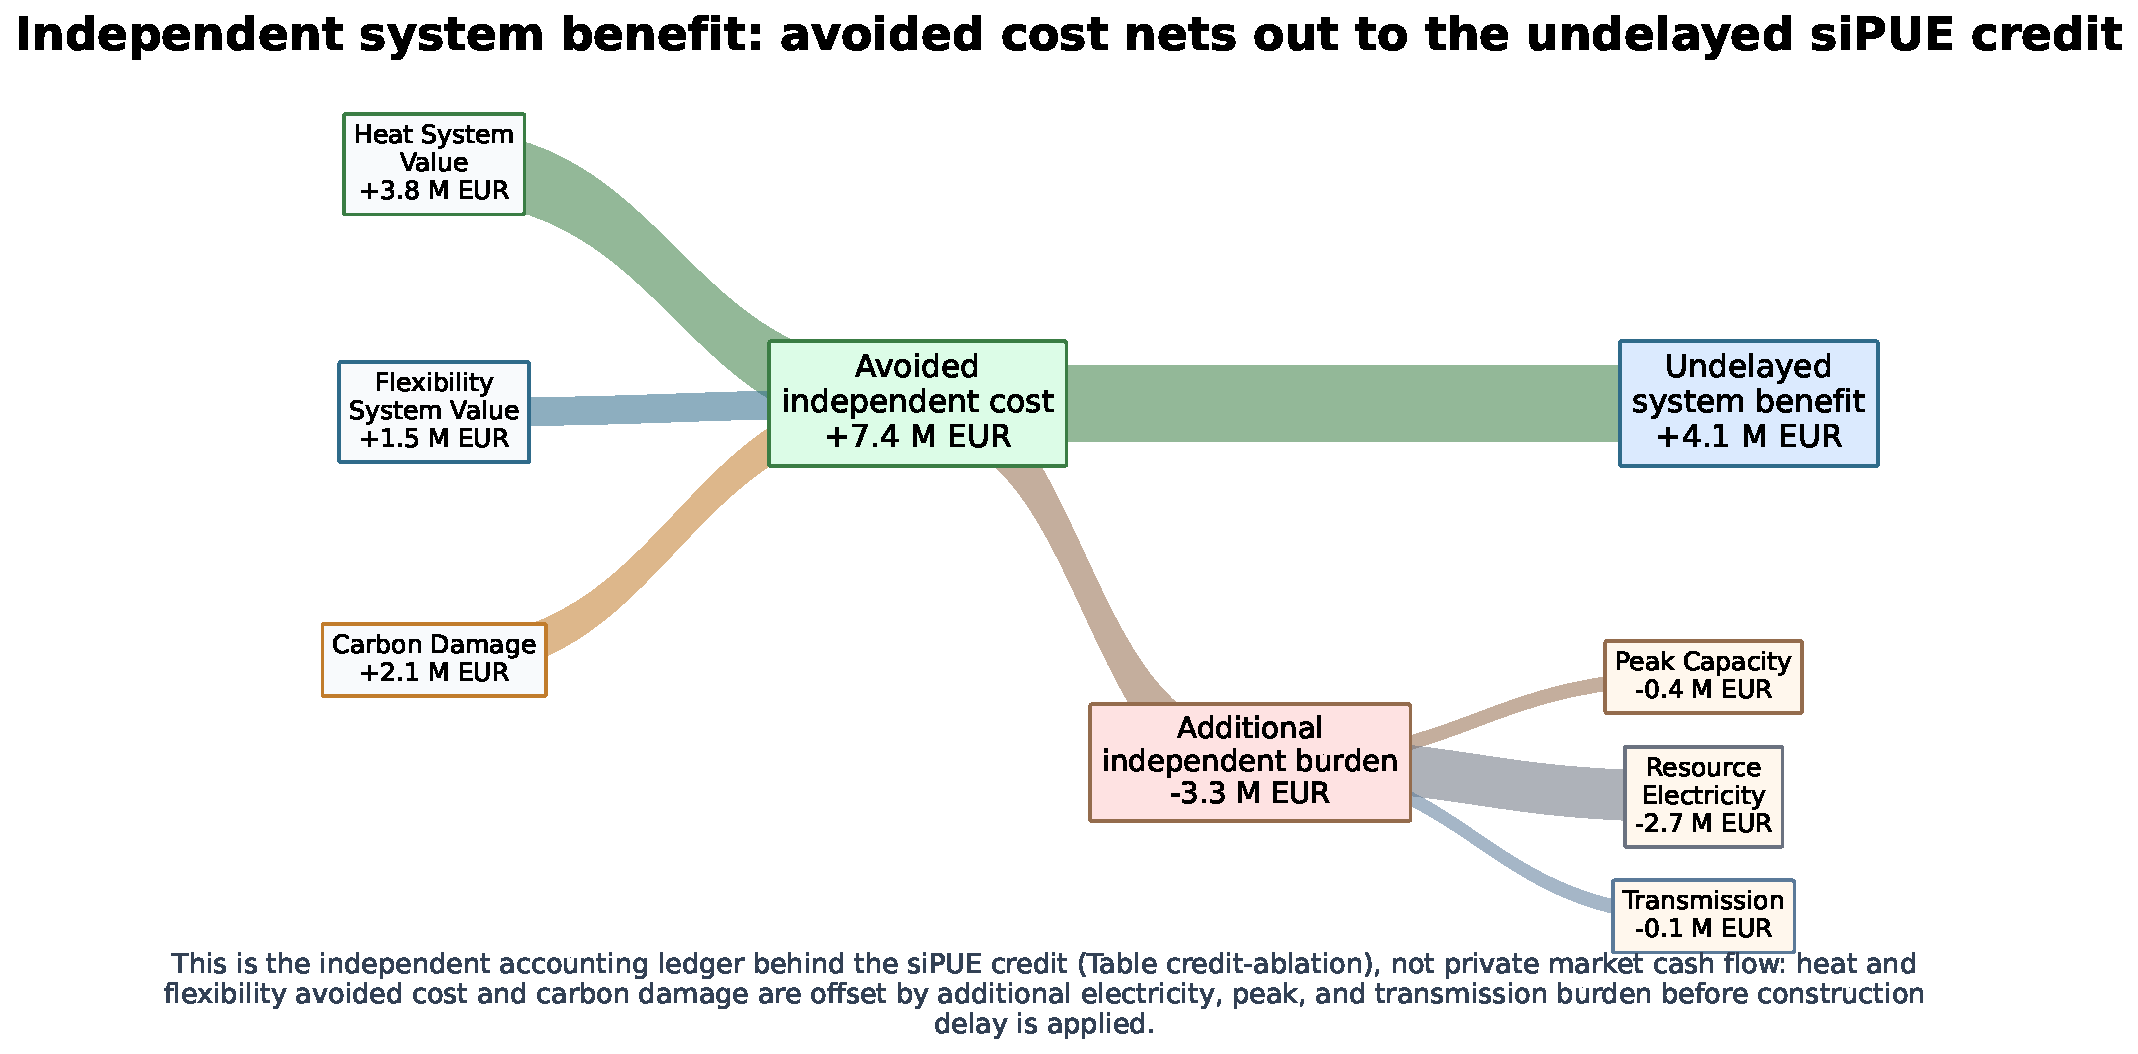
\includegraphics[width=0.95\linewidth]{fig_10_system_value_sankey.pdf}
\caption{System-value flow for the robust design. Heat and flexibility benefits are reported separately from electricity, carbon, capex, land, and delay adjustments.}
\label{fig:value-flow}
\end{figure}

\subsection{Carbon and delay accounting}

The model reports emissions, market carbon cost, carbon damage, avoided heat emissions, and power emissions as separate ledgers. This separation is important because carbon-damage valuation can change monetized system benefit without changing physical emissions. For that reason, carbon damage is retained as a ledger item and excluded from the main physical sensitivity factors.

\begin{table}[H]
\centering
\small
\caption{Carbon mechanisms and accounting treatment.}
\label{tab:carbon-mechanisms}
\begin{tabularx}{\linewidth}{L{3.0cm} X L{2.4cm} L{2.4cm}}
\toprule
Mechanism & Purpose & In optimization? & In siPUE credit? \\
\midrule
ETS payment & Private compliance and dispatch cost in the market ledger. & Yes & No \\
Carbon-damage value & External damage value in the independent accounting ledger. & Ledger only & Yes \\
Physical carbon cap & Row-level planning constraint shared by the fair services-disabled, baseline, robust, and scenario-perfect cases. & Yes & No direct monetary credit \\
\bottomrule
\end{tabularx}
\end{table}

\begin{figure}[H]
\centering
\begin{subfigure}{0.48\linewidth}
\centering
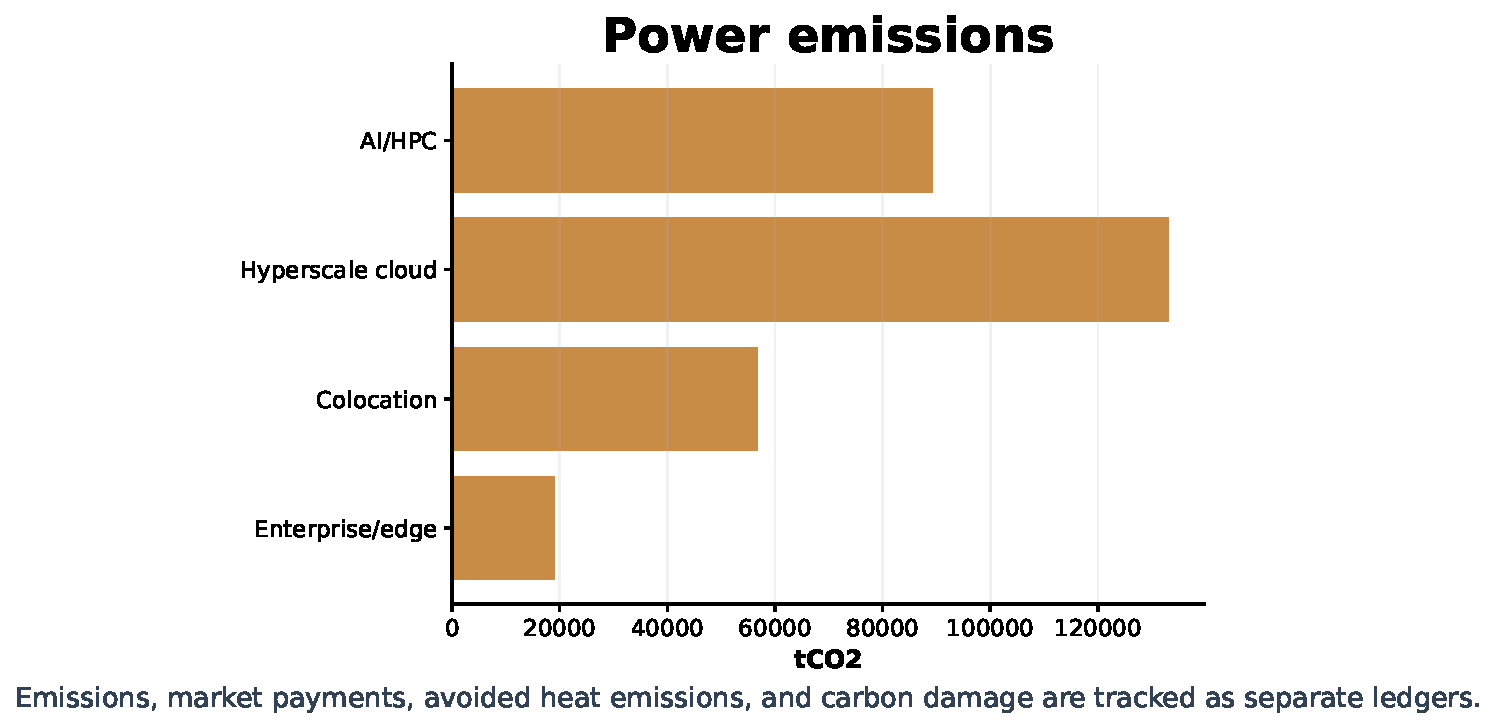
\includegraphics[width=\linewidth]{fig_11_carbon_ledger_power_emissions.pdf}
\caption{Power emissions.}
\end{subfigure}
\hfill
\begin{subfigure}{0.48\linewidth}
\centering
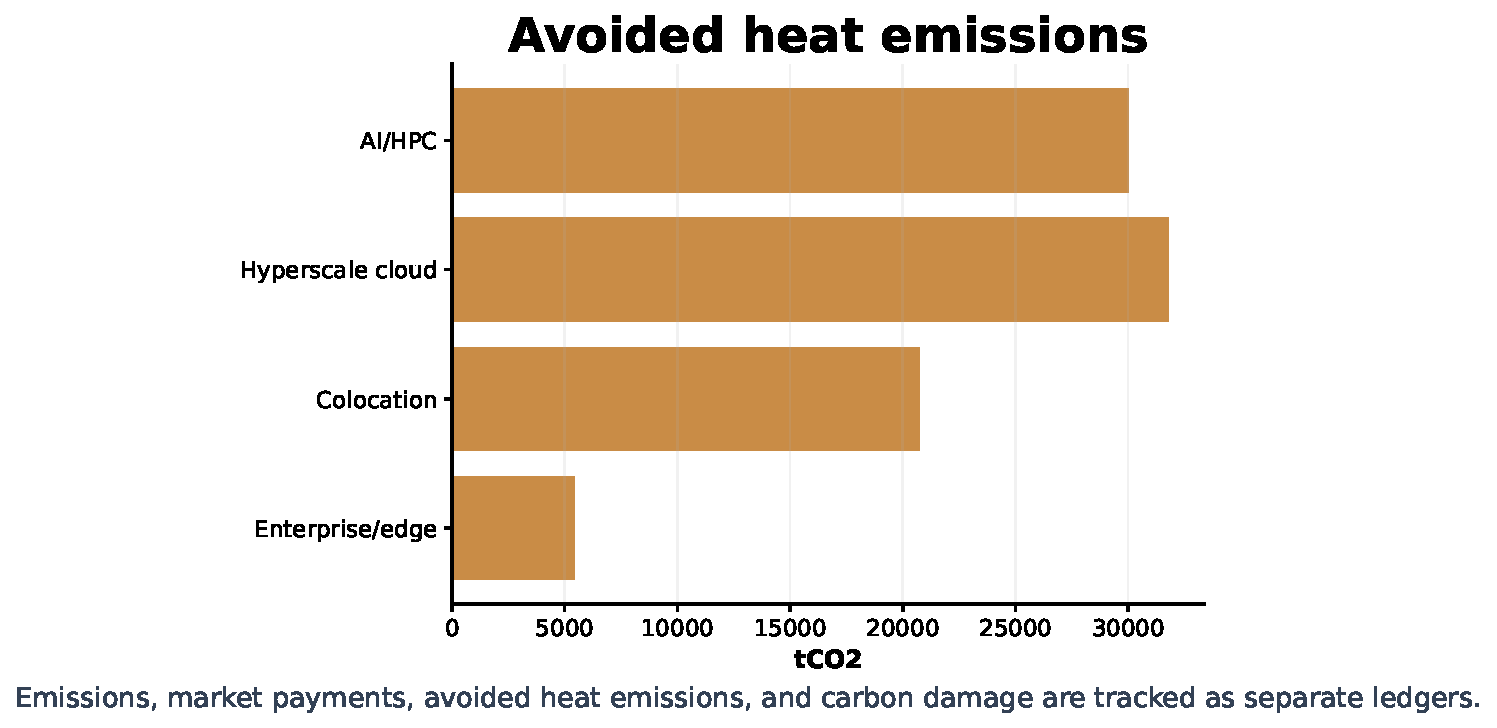
\includegraphics[width=\linewidth]{fig_11_carbon_ledger_avoided_heat_emissions.pdf}
\caption{Avoided heat emissions.}
\end{subfigure}
\caption{Carbon-ledger separation in the robust design.}
\label{fig:carbon-ledgers}
\end{figure}

Construction delay affects siPUE through the availability factor in Eq.~\ref{eq:sipue-credit}. It reduces the credit for useful system benefit while leaving the underlying facility energy accounting intact. The canonical outputs distinguish post-construction siPUE from delay-adjusted siPUE for this reason.

\begin{figure}[H]
\centering
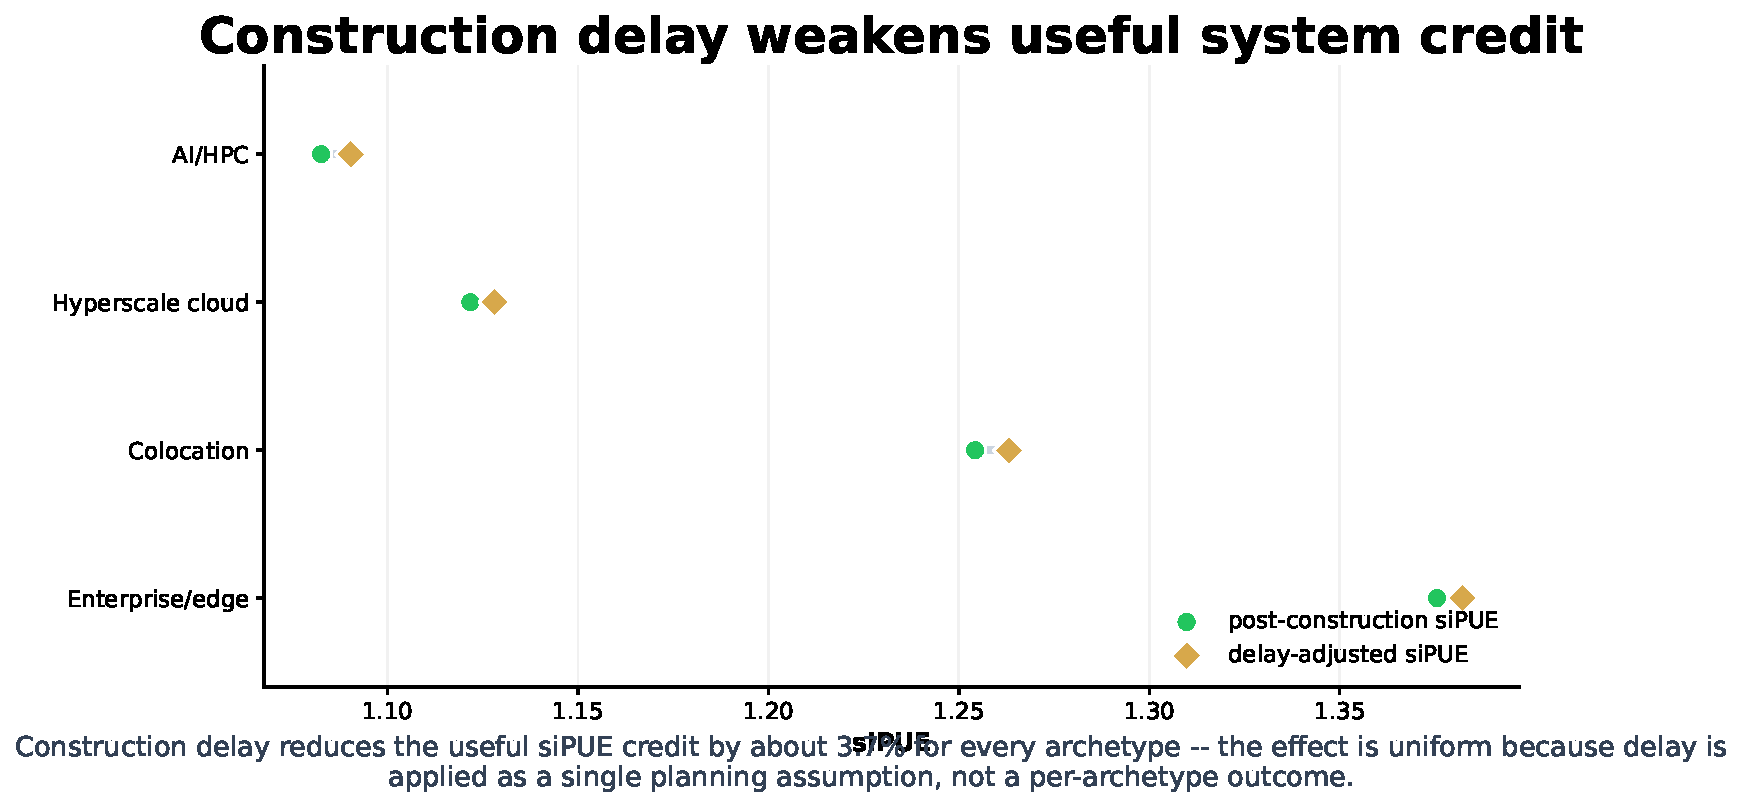
\includegraphics[width=0.86\linewidth]{fig_12_delay_credit_bridge.pdf}
\caption{Bridge from post-construction siPUE to delay-adjusted siPUE. Delay weakens the useful system credit before it enters the metric.}
\label{fig:delay-bridge}
\end{figure}

\subsection{Internal verification and robustness diagnostics}

The remaining results are diagnostics that qualify the headline claim: first checking the metric properties, then checking held-out and out-of-sample feasibility, and finally checking whether the cost-regret robust design would materially change if siPUE regret were optimized directly.

The results below are internal verification and robustness diagnostics; external validation requires observed projects. The property checks verify metric behavior: nonnegativity, no-services identity, delay weakening of credit, positive-benefit monotonicity, and ledger separation. The train/test diagnostic trains on earlier uncertainty states and evaluates held-out states. The out-of-sample diagnostic evaluates newly sampled states against the robust design.

\begin{figure}[H]
\centering
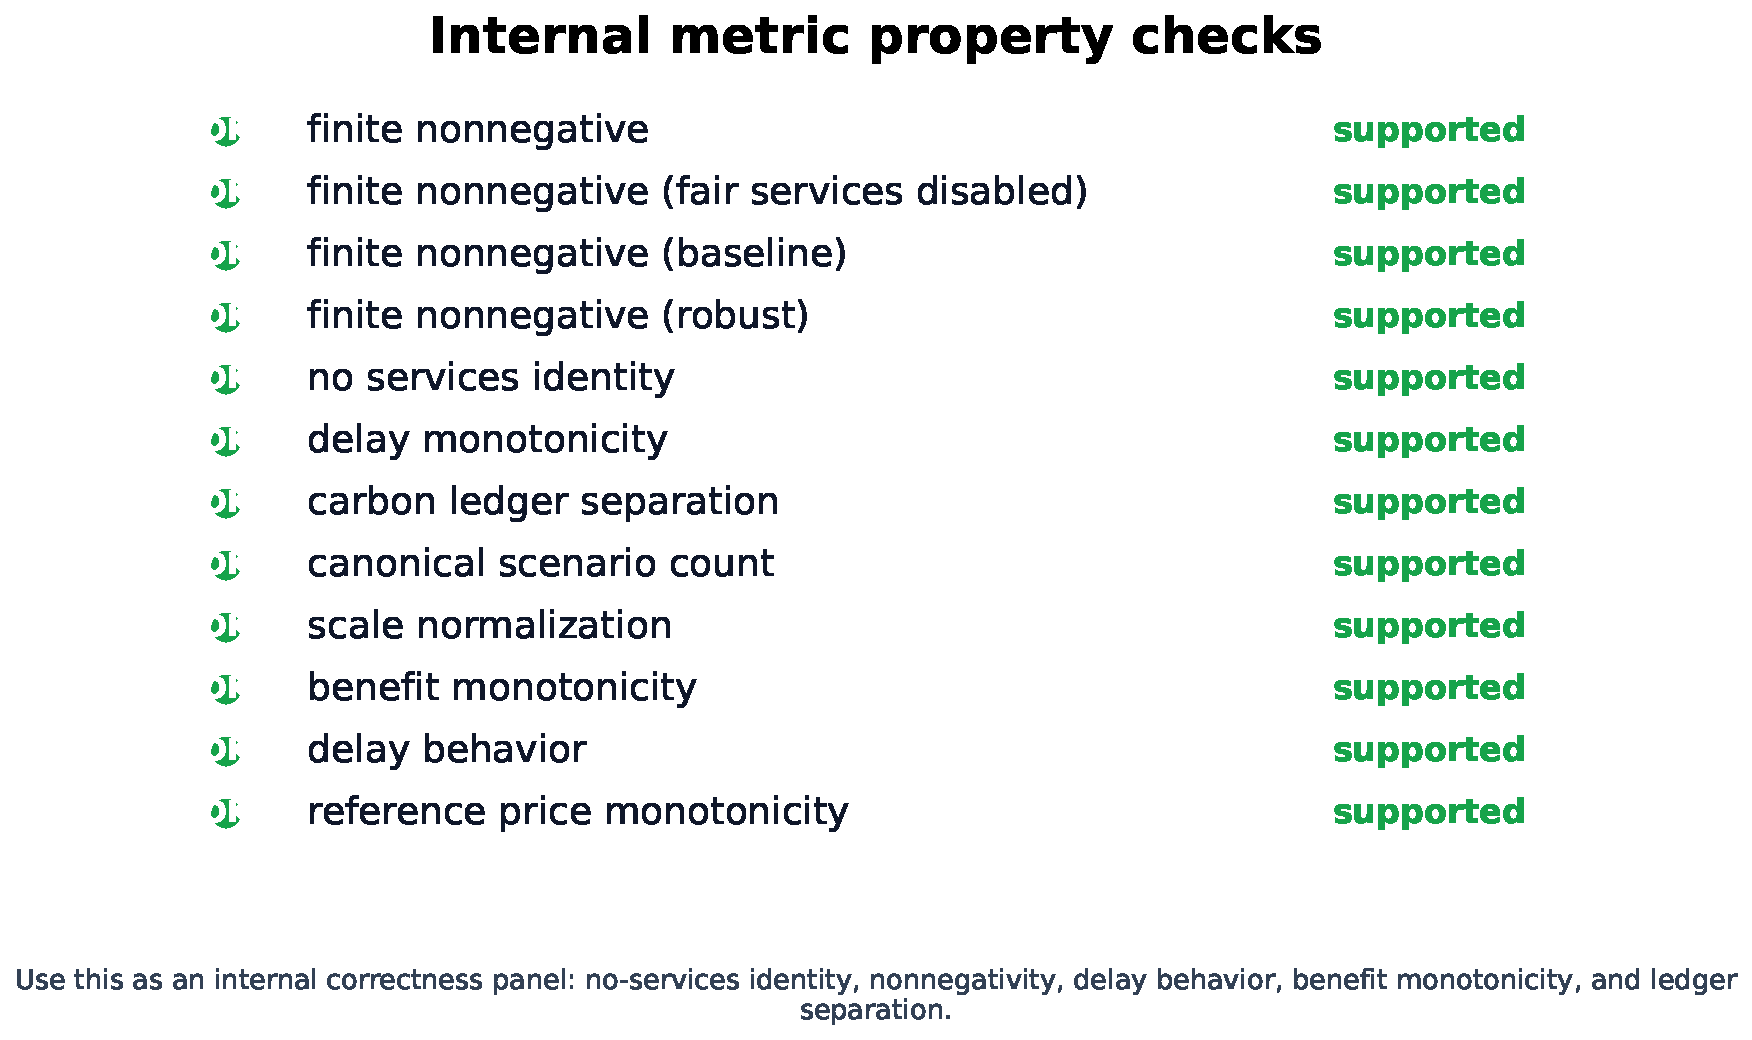
\includegraphics[width=0.92\linewidth]{fig_13_property_check_matrix.pdf}
\caption{Internal metric property checks: no-services identity, nonnegativity, delay behavior, benefit monotonicity, and ledger separation.}
\label{fig:property-checks}
\end{figure}

\begin{table}[H]
\centering
\small
\caption{Internal verification and robustness diagnostics. Regret is reported in EUR/MWh IT where comparable.}
\label{tab:validation-diagnostics}
\begin{tabular}{l r r r r}
\toprule
Diagnostic & Rows & Feasible rows & Mean regret & Regret range \\
\midrule
Train/test held-out & 12 & 12 & 1.065 & 0.013 to 4.170 \\
Out-of-sample & 40 & 40 & 0.402 & 0.012 to 1.241 \\
\bottomrule
\end{tabular}
\end{table}

The higher mean and wider range for train/test regret reflects how that diagnostic is constructed: the underlying design is trained on only 7 of the 10 canonical uncertainty states and evaluated against the 3 withheld states, including the highest-value ``service-upside'' state, which the design most under-provisions for. The out-of-sample diagnostic instead evaluates the design trained on the full 10-state set against independently sampled draws that rarely combine the same extremes, giving a lower and more stable regret.

\paragraph{siPUE headroom under cost-regret minimization} Stage~2 selects the robust design by minimizing worst-case normalized \emph{cost} regret (Eq.~\ref{eq:normalised-regret}); siPUE is computed after the design is selected, which raises the question of how much siPUE headroom this leaves on the table. Using the scenario-perfect benchmarks already computed for Stage~1, siPUE regret of the robust design against the scenario-specific, cost-minimizing optimum remains small relative to the headline fair-comparator shift. This comparison only bounds regret within the cost-optimal family, so we constructed the siPUE-optimizing alternative directly to test it.

\paragraph{Constructing the alternative directly} We therefore solved the alternative design problem directly. Stage~2 was re-solved with worst-case \emph{siPUE} regret against a per-scenario siPUE-perfect benchmark as the primary criterion, with the same lexicographic cost tie-break so the two runs are comparable side by side and differ only in the primary worst-case criterion. This required a matching Stage~1 siPUE-perfect benchmark, solved by minimizing siPUE for each scenario in isolation, using the same system-accounting ingredients as the siPUE credit itself so the two stages remain aligned. Inside both linear programs the siPUE-regret objective is built from the unclipped numerator $E_{\text{FAC}} - E_{\text{credit}}$, since the $[\cdot]^+$ operator in Eq.~\ref{eq:sipue} creates nonlinearity; realized siPUE is still reported with the clip applied. The two forms would diverge only if a design's unclipped numerator went negative; realized siPUE stays well above zero throughout this study. This affects the mathematical exactness of the siPUE-regret diagnostic in extreme cases, while the results reported here are unchanged. Table~\ref{tab:sipue-objective-comparison} compares the resulting shared design against the canonical cost-regret robust design for the same 40 rows.

\begin{table}[H]
\centering
\small
\caption{Cost-regret-minimizing (canonical robust) design versus siPUE-regret-minimizing design, by archetype. Worst-case regret is the maximum, within each archetype's shared 10-scenario group, of siPUE for that design minus the scenario-perfect siPUE benchmark. Average cost is the mean lifecycle market cost (NPV, EUR) across the same 10 rows.}
\label{tab:sipue-objective-comparison}
\begin{tabular}{l r r r r}
\toprule
Archetype & Worst regret & Worst regret & Avg. cost & Design \\
 & (cost-regret) & (siPUE-regret) & difference & identical? \\
\midrule
AI/HPC & 0.0656 & 0.0683 & $-0.002\%$ & No \\
Hyperscale cloud & 0.0438 & 0.0476 & $-0.002\%$ & No \\
Colocation & 0.0418 & 0.0418 & $0.00\%$ & Yes \\
Enterprise/edge & 0.0243 & 0.0243 & $0.00\%$ & Yes \\
\bottomrule
\end{tabular}
\end{table}

For two of the four archetypes, Colocation and Enterprise/edge, minimizing worst-case siPUE regret directly selects the \emph{exact same} shared design, capacity for capacity, as minimizing worst-case cost regret. For AI/HPC and Hyperscale cloud, the objectives diverge modestly. Averaged across all 40 canonical rows and weighted by each archetype's annual IT energy, mean siPUE is 1.1519 under cost-regret minimization and 1.1532 under siPUE-regret minimization; mean PUE is 1.3431 versus 1.3483. The siPUE difference, 0.0013, is small next to the fair-comparator-to-robust shift in Table~\ref{tab:kpi-summary}. Some of this closeness likely reflects the problem structure as well as this parameterization: the market-cost objective and the independent accounting ledger behind siPUE share several underlying price and cost terms, so the two Stage~2 criteria are partly coupled.

\paragraph{Out-of-sample confirmation} The comparison above trains and evaluates both Stage-2 objectives on the same ten canonical uncertainty states used throughout this paper, which leaves open whether the near-identical designs persist under fresh scenarios. We repeated the comparison end to end -- both Stage-1 benchmarks and both Stage-2 objectives, re-solved from scratch -- on 40 freshly drawn uncertainty scenarios (10 per archetype) outside the canonical design set. On this out-of-sample draw, three of four archetypes select the identical design under the two objectives; AI/HPC differs slightly. The IT-energy-weighted mean siPUE is 1.1793 under cost-regret minimization and 1.1786 under siPUE-regret minimization, and mean PUE is 1.3466 versus 1.3463. This provides a fresh-scenario diagnostic beyond the in-sample result, while still remaining internal to the same scenario-generation structure.

\begin{figure}[H]
\centering
\begin{subfigure}{0.48\linewidth}
\centering
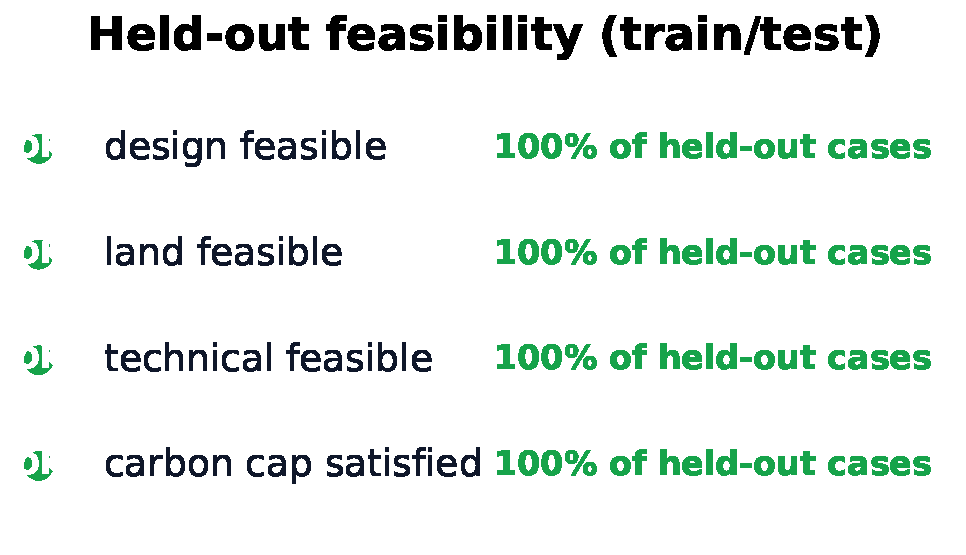
\includegraphics[width=\linewidth]{fig_14a_train_test_feasibility.pdf}
\caption{Train/test feasibility.}
\end{subfigure}
\hfill
\begin{subfigure}{0.48\linewidth}
\centering
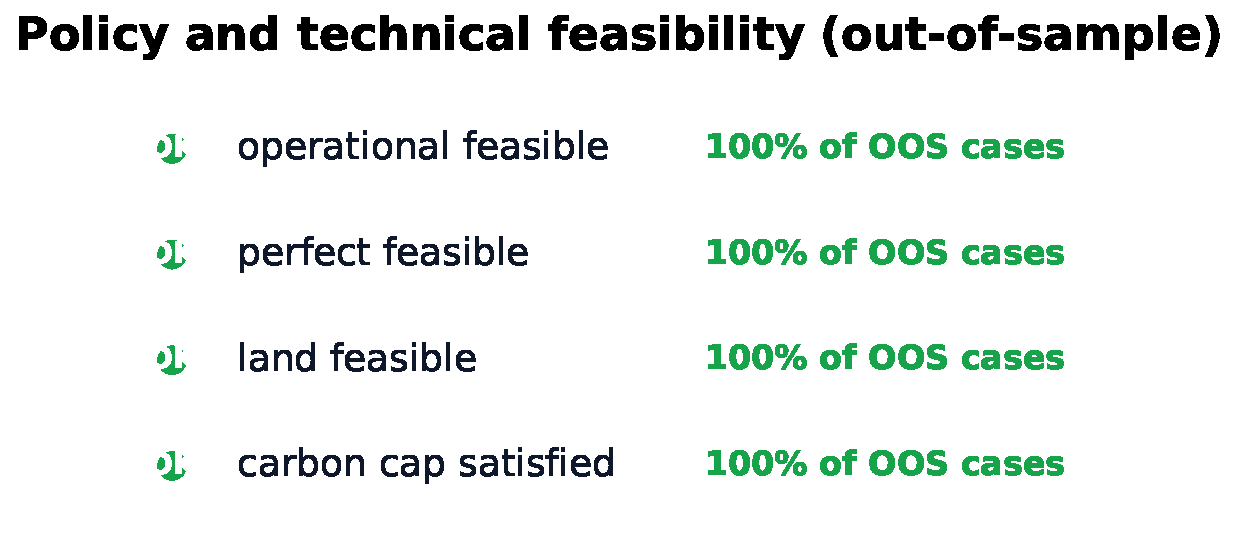
\includegraphics[width=\linewidth]{fig_15a_out_of_sample_feasibility.pdf}
\caption{Out-of-sample feasibility.}
\end{subfigure}
\caption{Feasibility diagnostics for held-out and out-of-sample cases.}
\label{fig:validation-feasibility}
\end{figure}

\begin{figure}[H]
\centering
\begin{subfigure}{0.48\linewidth}
\centering
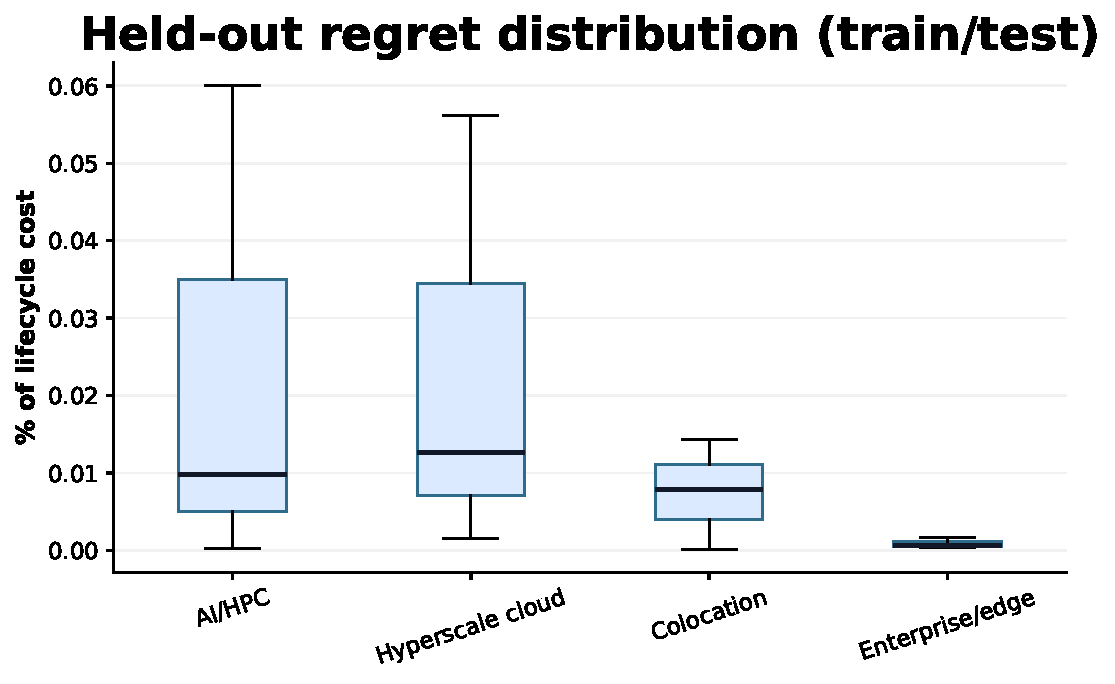
\includegraphics[width=\linewidth]{fig_14b_train_test_regret.pdf}
\caption{Train/test regret.}
\end{subfigure}
\hfill
\begin{subfigure}{0.48\linewidth}
\centering
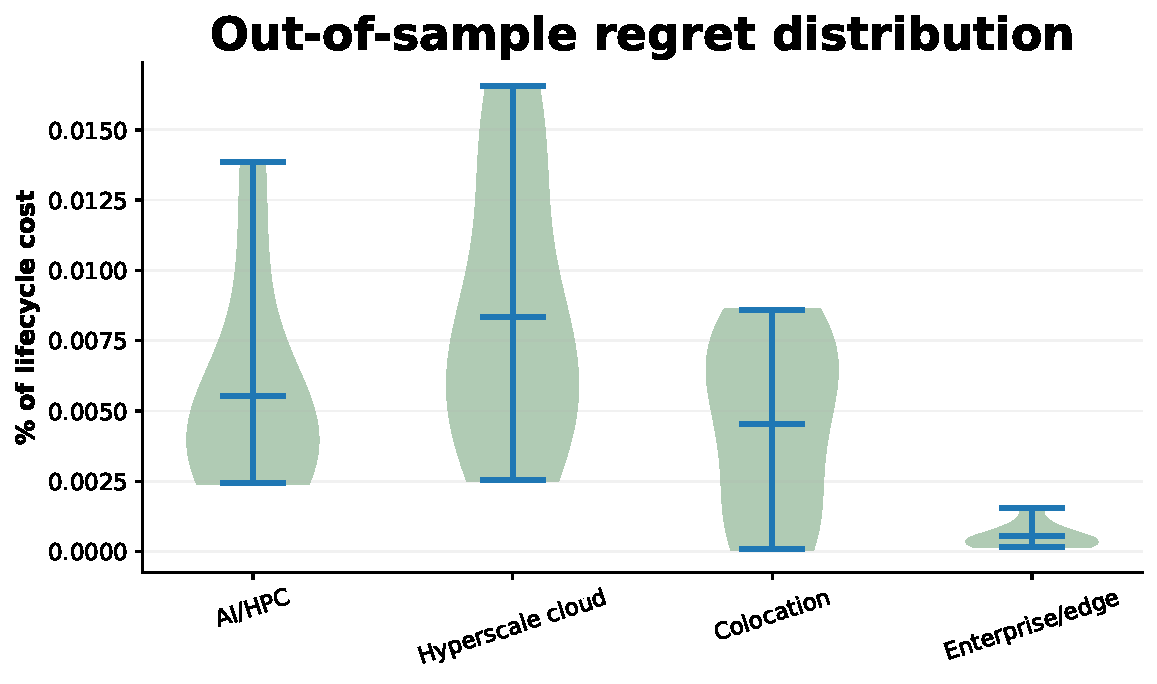
\includegraphics[width=\linewidth]{fig_15b_out_of_sample_regret.pdf}
\caption{Out-of-sample regret.}
\end{subfigure}
\caption{Regret diagnostics for held-out and out-of-sample cases, complementing the feasibility panels above and the summary statistics in Table~\ref{tab:validation-diagnostics}.}
\label{fig:validation-regret}
\end{figure}

\subsection{Sensitivity analysis}

The manuscript sensitivity varies five factors: heat price, flexibility price, cooling overhead, land availability, and construction delay. Carbon damage is excluded from this sensitivity set because it is a valuation ledger, while the sensitivity set is reserved for physical design and delivery levers. Congestion, battery-ceiling, and regret-surface diagnostics are also excluded from the final manuscript sensitivity set.

\begin{table}[H]
\centering
\small
\caption{All-archetype sensitivity results for the robust design across the 40-row scenario set for each sensitivity case, weighted by each archetype's annual IT energy.}
\label{tab:sensitivity-summary}
\begin{tabularx}{\linewidth}{L{2.5cm} L{2.25cm} r r r r}
\toprule
Factor & Level & PUE & siPUE & Benefit & Land use \\
 & & & & (EUR/MWh IT) & (\%) \\
\midrule
Canonical & base & 1.343 & 1.152 & 10.825 & 75.2 \\
Heat price & low & 1.239 & 1.117 & 6.895 & 60.4 \\
Heat price & high & 1.365 & 1.161 & 11.554 & 79.9 \\
Flexibility price & low & 1.344 & 1.171 & 9.840 & 73.1 \\
Flexibility price & high & 1.342 & 1.150 & 10.907 & 75.8 \\
Cooling overhead & low & 1.308 & 1.118 & 10.750 & 74.4 \\
Cooling overhead & high & 1.378 & 1.186 & 10.898 & 75.9 \\
Land availability & low & 1.316 & 1.163 & 8.696 & 96.5 \\
Land availability & high & 1.343 & 1.152 & 10.825 & 62.6 \\
Land availability & unconstrained & 1.343 & 1.152 & 10.825 & 0.8 \\
Construction delay & 0 months & 1.347 & 1.146 & 11.403 & 76.9 \\
Construction delay & 12 months & 1.343 & 1.161 & 10.279 & 74.9 \\
\bottomrule
\end{tabularx}
\end{table}

The sensitivities should be read through the same two-part logic: a physical facility-energy channel and a monetary value-credit channel. Cooling overhead acts mainly through facility energy and therefore moves both PUE and siPUE. Flexibility price acts mainly through system benefit and changes siPUE more than PUE. Heat price can affect both channels because each sensitivity is re-optimized with its own dispatch; a higher heat price can induce a more energy-intensive service portfolio, so siPUE can move irregularly with heat value. Construction delay weakens the value credit. Low land availability binds in three all-scenario robust cases and reduces system benefit, but the land model remains stylized.

\begin{figure}[H]
\centering
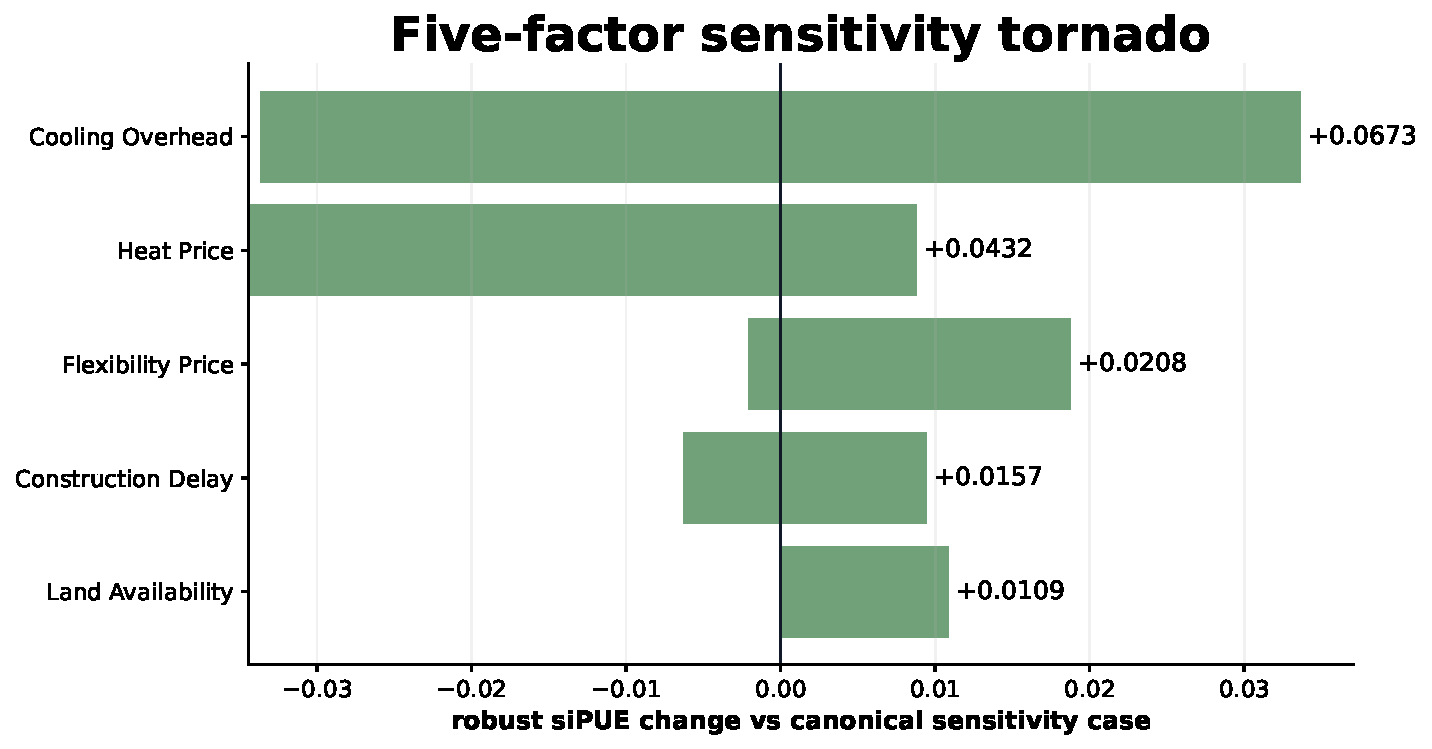
\includegraphics[width=0.88\linewidth]{fig_17_sensitivity_tornado.pdf}
\caption{Five-factor sensitivity tornado for robust siPUE. Carbon damage is excluded from the sensitivity factors.}
\label{fig:sensitivity-tornado}
\end{figure}

\begin{figure}[H]
\centering
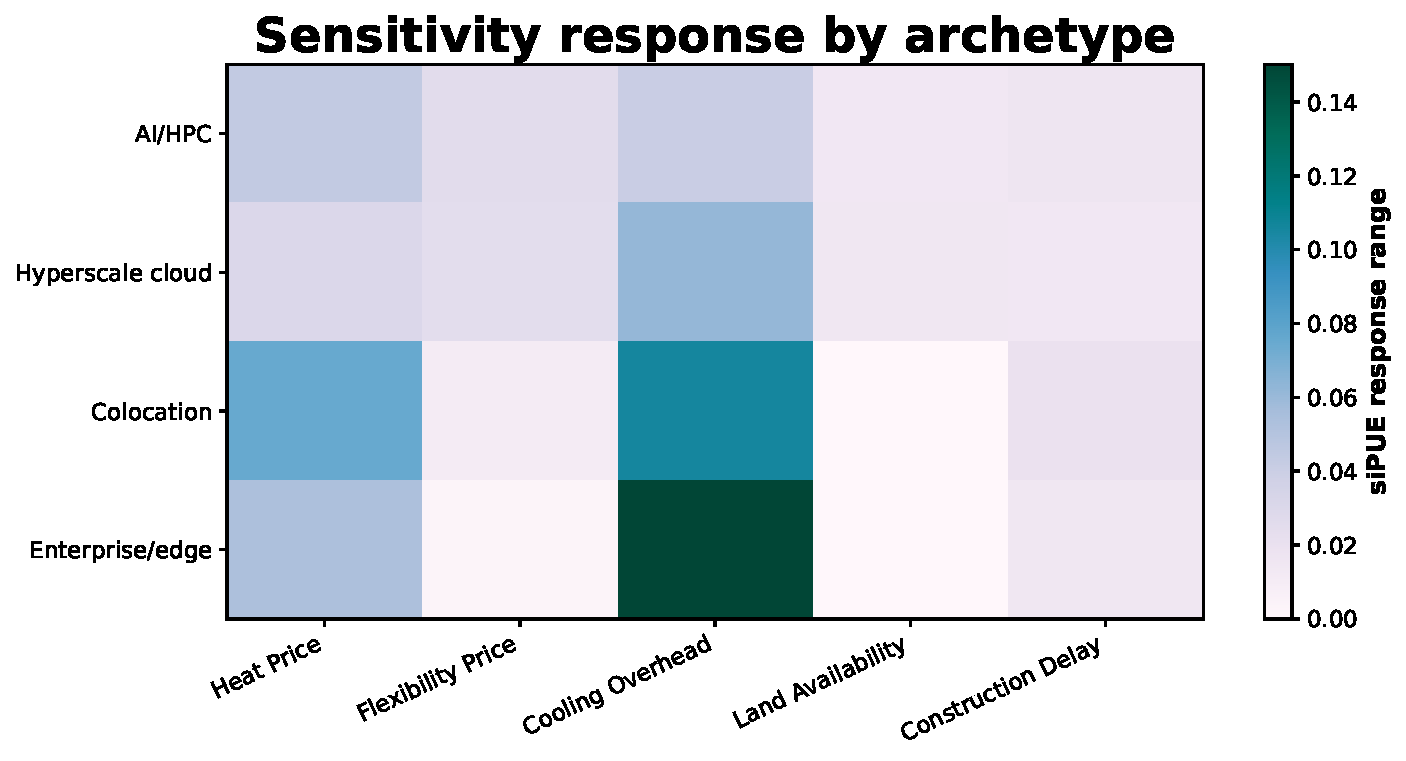
\includegraphics[width=0.92\linewidth]{fig_18_sensitivity_archetype_response.pdf}
\caption{Sensitivity response by archetype.}
\label{fig:sensitivity-archetype}
\end{figure}

\subsection{Face validity against published benchmarks}
\label{sec:face-validity}

The diagnostics above are internal. This subsection adds a narrower, external check: whether the model's modeled PUE and heat-reuse levels are in a plausible range next to published, real-project figures \cite{UptimeInstitute2024Survey,EUSmartCities2024Mantsala}. The comparison is used for face validity, and no model parameter is fit to the figures below.

For PUE, the Uptime Institute's 2024 global survey reports an industry-average PUE of 1.56--1.58, with hyperscale operators (Google, Amazon Web Services, Microsoft) claiming 1.2 or lower at some sites, and new-build large colocation campuses commonly targeting around 1.4 \cite{UptimeInstitute2024Survey}. The no-services (pure facility-overhead, zero efficiency investment) PUE in the canonical archetypes is 1.12 for AI/HPC and 1.18 for Hyperscale cloud, both inside the published hyperscale range. Colocation (1.30) and Enterprise/edge (1.42) sit below the published industry-wide average of 1.56--1.58, closer to what only modern, newly built facilities achieve. This reflects the intended scope: the archetypes represent facilities capable of considering integration investment, which skews toward the newer, more efficient end of the real fleet.

For heat reuse, the Mäntsälä data center in Finland operates a dedicated 4.0~MW heat pump and reuses 75\% of its energy as district heat, a real, purpose-built, single-service case \cite{EUSmartCities2024Mantsala}. In this study, delivered useful heat divided by modeled facility electricity reaches 0.30--0.33 for AI/HPC and Colocation and 0.22--0.26 for Hyperscale cloud and Enterprise/edge, well below the Mäntsälä figure. This ratio is used as a face-validity output and remains outside official Energy Reuse Factor accounting. The modeled archetypes are general-purpose facilities that size heat recovery as one constrained service among several. Heat, flexibility, storage, land, and construction-delay exposure all compete for the same capital. This scope explains the gap to a single-purpose heat-export site. The effective recoverable-heat-fraction inputs span 0.17--0.575 after state multipliers, but capacity sizing, district-heating demand, pipe limits, and cost trade-offs still bind delivered heat below the dedicated project benchmark.

Table~\ref{tab:face-validity} summarizes both comparisons. Both directions of mismatch (PUE running better than the published average; heat-delivery intensity running below a dedicated best-practice site) are consistent with the archetypes' intended scope and bound how far the numerical results in this paper should be extrapolated to a specific real facility.

\begin{table}[H]
\centering
\small
\caption{Face validity of modeled PUE and heat-reuse levels against published, real-project figures.}
\label{tab:face-validity}
\begin{tabularx}{\linewidth}{l X X}
\toprule
Quantity & Published reference & Modeled range (this study) \\
\midrule
Hyperscale/AI PUE & 1.1--1.2 at leading sites \cite{UptimeInstitute2024Survey} & 1.12--1.18 (no-services) \\
Colocation/enterprise PUE & 1.4 (new-build) to 1.56--1.58 (industry average) \cite{UptimeInstitute2024Survey} & 1.30--1.42 (no-services) \\
Delivered useful heat / facility electricity & 0.75 at a dedicated site (M\"ants\"al\"a) \cite{EUSmartCities2024Mantsala} & 0.22--0.33 (robust design output) \\
\bottomrule
\end{tabularx}
\end{table}

\subsection{Limitations and future work}

Several limitations define the scope of the results. The model is a controlled testbed for metric behavior; site forecasting would require project-specific input data and calibration. The absolute NPV values, capacity choices, and KPI levels should therefore be read as outputs of a stylized comparison. Project-specific prediction would require a local investment model. The three-node network is useful for consistent DC-OPF accounting, while local grid assessment would require an interconnection study. Representative days reduce the annual operating problem to a tractable form and omit some operational extremes. The land constraint is a lease or opportunity-cost representation used for comparative modeling. The independent system-cost values used in siPUE should also be replaced with local values before applying the metric to a real investment case.

These limits restrict the interpretation of the numerical results while leaving the central metric claim intact. The evidence supports the accounting argument that PUE can penalize service-active designs because it observes facility electricity without observing separately accounted local-system benefits. Site-level claims about siPUE, heat reuse, or lifecycle cost require observed project data. Some archetype-specific conclusions remain evidence gaps, especially hyperscale flexibility, enterprise/edge flexibility, and enterprise/edge heat recovery.

The current model excludes water use, embodied carbon, formal Renewable Energy Factor, and official ISO Energy Reuse Factor accounting \cite{ISO30134,EUDataCenterDirective2023}. It also treats flexibility as reserve availability, with activated scarcity events left for future validation. Section~\ref{sec:face-validity} adds a plausibility check against aggregate published PUE and heat-reuse figures \cite{UptimeInstitute2024Survey,EUSmartCities2024Mantsala}. Future work should add observed project data at the transaction level, richer network models, water and embodied-carbon ledgers, contracting structures between data centers and utilities, activation-event validation for reserve delivery, and external validation against measured heat and flexibility transactions.

\section{Conclusion}

This paper connects a contextual policy and market synthesis of data centers in local energy systems with a structured method for evaluating system-integrated designs. The proposed siPUE indicator is a PUE-compatible companion indicator that converts separately accounted local-system benefits, including heat, flexibility, peak, carbon damage, and delay, into an energy-equivalent numerator credit. The metric reduces to PUE when no services are active, which preserves backward compatibility with existing reporting.

The 40-row canonical analysis supports a value-channel interpretation, but with narrower claims than a no-services-only counterfactual would support. Reported averages weight each archetype by its annual IT energy. The identity no-services case verifies that PUE and siPUE are both 1.196 when service capacity and efficiency investment are zero. The fair services-disabled comparator has PUE and siPUE of 1.167 under the same locked efficiency retrofit and carbon-cap treatment used for the service-active cases. Relative to that comparator, the baseline design raises average PUE to 1.238 and lowers siPUE to 1.139; the robust design raises PUE to 1.343 and lowers siPUE to 1.152. Baseline creates 5.603~EUR/MWh IT of delay-adjusted system benefit and robust creates 10.825~EUR/MWh IT. The credit-to-burden ratio falls from about 1.40 for baseline to 1.08 for robust, consistent with diminishing marginal system value. At the row level, siPUE falls below the fair services-disabled comparator in 36 of 40 baseline rows and 23 of 40 robust rows.

The compact metric benchmark supports paired reporting of PUE and siPUE. PUE measures internal facility overhead \cite{Belady2008PUE,greengrid2014,ISO30134}. Carbon, heat, and emissions remain separate ledgers. siPUE translates separately accounted system benefit into the same energy-normalized language as PUE, making the burden-and-value trade visible while preserving the distinction from thermodynamic efficiency. The carbon-damage ledger is important: excluding carbon damage raises robust siPUE above the fair services-disabled comparator on average, so the empirical result is conditional on the stated social-carbon valuation.

Internal verification and robustness diagnostics support numerical consistency, not external validation. The no-services identity, nonnegativity, delay behavior, benefit monotonicity, and ledger separation checks are satisfied. Train/test and out-of-sample diagnostics remain feasible and show nonnegative comparable regret. Re-solving Stage~2 with worst-case siPUE regret instead of cost regret changes the IT-energy-weighted in-sample average siPUE by 0.0013 and the out-of-sample average by -0.0007. A face-validity comparison against published PUE and heat-reuse figures \cite{UptimeInstitute2024Survey,EUSmartCities2024Mantsala} places the modeled ranges inside or near the published range for hyperscale facilities, on the more efficient side of the published range for colocation and enterprise sites, and below a dedicated best-practice heat-reuse site, consistent with the archetypes' intended scope. The flexibility credit should be read as reserve-availability accounting, with activated reserve delivery under scarcity events left outside the current validation scope.

The practical implication is simple: a data center can look worse under PUE when it becomes more useful to the local energy system. PUE remains useful for internal facility overhead, while paired siPUE reporting adds the local-system value channel. siPUE should therefore be reported next to PUE, using explicit limits, explicit inputs, and a clear services-disabled comparator to show whether separately accounted local-system benefits are large enough to account for the extra facility energy.

\section*{Declaration of competing interest}

The authors declare that they have no known competing financial interests or personal relationships that could have appeared to influence the work reported in this paper.

\section*{Data availability}

The data and results underlying this study are available in the same BRAVE GitHub repository as the code (see Code availability below).

\section*{Code availability}

The computational implementation supporting this study is available in the BRAVE GitHub repository:
\url{https://github.com/sambeets/BRAVE/tree/main/sipue_modelling}. 
 

\section*{Acknowledgement}
This research has received financial support from Interreg project BRAVE, and FME RenewHydro (Grant 350468, Research Council of Norway).
\IfFileExists{brave.pdf}{
\begin{figure}[H]
\raggedright
\includegraphics[width=0.5\linewidth]{brave.pdf}
\end{figure}
}{}


%%%%%%%%%%%%%%%%%%%%%%%%%%%%%%%%%%%%%%%%%%%%%%%%%%%%%%%%%%%%%%%%%%%%%%%%%%%%%%55

\bibliographystyle{elsarticle-num-names}
\bibliography{references}

\end{document}
